\documentclass[11pt,a4paper,oneside]{mythesis_mtr}

\usepackage{lscape}
\usepackage[round]{natbib}
%\usepackage{subfigure}
\usepackage{graphicx}
\usepackage{mathptm}
\usepackage{amsmath}
\usepackage{latexsym,flafter,afterpage,amssymb,color}
\usepackage{verbatim}
\usepackage{rotating}
\usepackage{setspace}
\usepackage{caption}
\usepackage{subcaption}
\doublespacing

% Use Adobe Times Roman (for printing)
%\renewcommand{\rmdefault}{ptm}
\usepackage{palatino}
%\usepackage{doublespace}

% Multicolumns in tables, shading in tables,tables to appear over multiple pages
\usepackage{multirow,colortbl,longtable}



% Page setup
\topmargin=-0.41in
\textwidth=6.5in%6.5
\textheight=9.8in
\headsep=24pt
\oddsidemargin=4mm
\parindent=0.3in
\parskip=0.1in

\newlength{\rulewidth}
\setlength{\rulewidth}{6.5in} % change to 150mm for printing on
                  % gordon, 149 otherwise???

\pagestyle{headings}

\setcounter{secnumdepth}{5}              %Numbers subsubsections, and lower.
\setcounter{tocdepth}{5}                 %Sets depth of toc to include subsubsections.



% bibliography is in a folder
%\newcommand{\BIB}{/home/swr06rsc/Documents/latex}
\newcommand{\BIB}{..}

% a bunch of useful shortcuts

\newcommand{\deriv}[2]{\frac{d #1}{d #2}}
\newcommand{\pderiv}[2]{\frac{\partial #1}{\partial #2}}
\newcommand{\tderiv}[2]{\frac{D #1}{D #2}}
\newcommand{\vect}[1]{{\bf #1}}
\newcommand{\pd}[2]{\frac{\partial^2 #1}{\partial #2^2}}

%\textwidth=149mm

\sloppy

% 1.5 line spacing so my supervisor can scrawl all over it
\renewcommand{\baselinestretch}{1.5}

% Tell latex not to mind if 0.75 of a page is full of floats
%\renewcommand{\floatpagefraction}{0.99}

% Text to put in the header

%\makeglossary

\begin{document}


\pagenumbering{roman}
%Title page

\begin{titlepage}
\begin{flushright}
\begin{figure}[h]
\begin{flushright}
  \vspace{-2cm}
\includegraphics[width=50mm]{preface/figures/reading_logo.pdf} %pdf for use with pdflatex
\end{flushright}
\end{figure}
\end{flushright}
\begin{flushleft}
  \vspace{4cm}
\Huge{\bf{Title}}\\ %title of PhD
\huge{PhD in Atmosphere, Oceans and Climate} \\ %PhD course
\Large{\bf{Department of Meteorology}}\\ %Department
\vspace{2cm}
\huge{Emma Dodd} \\ %name
\Large{\bf{November 2014}}\\ %submission date
\end{flushleft}
\end{titlepage}

\thispagestyle{empty}
%---------------------------------------------------------------------------

% Declaration

\vspace{40mm}
\chapter*{\centering \Large \vspace{-20mm}\Huge Declaration}
\thispagestyle{headings}

\par I confirm that this is my own work and the use of all material from other sources has been properly and fully acknowledged.

\vspace*{2cm}
- Emma Dodd %\hspace{3.75in}

\newpage
\thispagestyle{empty}
%----------------------------------------------------------------------------

%The abstract.

\chapter*{\centering \Large \vspace{-20mm}\Huge Abstract}
\thispagestyle{headings}

Abstract goes here

%----------------------------------------------------------------------------
%Acknowledgements
\chapter*{\centering \Large \vspace{-20mm}\Huge Acknowledgements}
\thispagestyle{headings}

Acknowledgements go here.


\vspace{2cm}

%- Robert Lee - December 2013

\newpage
\thispagestyle{empty}
%----------------------------------------------------------------------------

\tableofcontents

%------------------------------------------------------------------------------

\pagenumbering{arabic}

%\begin{document}

\chapter{Introduction}
\label{chap:intro}
\thispagestyle{headings}
\section{Motivations and aims of the thesis}
\label{chap:intro_motivations}
Motivations / examples of storms and why its relevant to research how they might change in the future.\\
Aims and set of key scientific questions.
\section{Extratropical storm tracks}
\label{chap:intro_lit_tracks}
Talk a bit



\chapter{Method and Tools}
\label{chap:method}
\thispagestyle{headings}
\documentclass[11pt]{article}
\usepackage[sort]{natbib}
\usepackage{bm,amsmath,bbm,amsfonts,nicefrac,latexsym,amsmath,amsfonts,amsbsy,amscd,amsxtra,amsgen,amsopn,bbm,amsthm,amssymb,graphicx, breqn, setspace, printlen, caption, subcaption, pbox, fixltx2e, bm}
\usepackage{fancyhdr, color}
\usepackage{mathptmx, placeins}     
\bibliographystyle{abbrvnat}
%\usepackage[section]{placeins}
\usepackage[margin=1.0in]{geometry}

\title{Observability and information content {\color{red}DRAFT}}
\author{Ewan Pinnington}

\newtheorem{theorem}{Theorem}[section]
\newtheorem*{defn}{Definition}


\begin{document}

\maketitle

\section{Introduction}
In data assimilation it is important to understand if the observations available to us provide us with enough information to find a meaningful description of our studied system. Measurements of forest carbon balance are now routinely made in forests across the world using micrometeorological techniques, with many other relevant observations such as leaf area index and standing biomass also available \citep{baldocchi2008turner}. Many efforts have been made to combine this data with models of forest carbon balance using data assimilation techniques in order to improve modelled estimates \citep{zobitz2011primer, fox2009reflex, richardson2010estimating, Quaife2008, Zobitz2014, Niu2014}. Currently, however, the relative levels of information from different data types is not well understood. 

In numerical weather prediction many measures of observation information content have been defined \citep{Cardinali2004, rodgers2000inverse, fisher2003estimation}. These measures can be used to identify how information content might vary both temporally and spatially, when observations are made at different times or in different locations. It is not necessary to have made a physical observation in order to estimate its information content. It is enough to have an accurate estimate to the observation error at the specified time and location. It is therefore possible to use these measures to define target observations or design new observing systems \citep{palmer1998singular, eyre1990information}. Often we are required to know the derivative of our model in order to implement these measures. This can prove difficult to implement. However, techniques such as automatic-differentiation \citep{renaud1997automatic} can reduce the time taken to find the derivative of a model.  

In this chapter we aim to analyse the information content in the observations used for assimilation with the DALEC1 and DALEC2 models of ecosystem carbon balance. We begin by considering the observability of our system given a set of observations. Observability is a mathematical concept from control theory. Applied to data assimilation a system is defined as observable if for a given set of observations we can uniquely define the initial state for our model. This allows us to determine if from current observations used in carbon balance data assimilation, we have enough information to find a unique model state. In practice we include a background term in our assimilation ({\color{red}ref. DA section}) to ensure we can always find a locally unique solution. However, it is informative to show that observations alone provide us with enough information to find a unique solution.

We then consider different information content measures applied to our system in order to show how the information content varies for the different observation types available to us for DALEC1. We then extend these results to the DALEC2 model and investigate how the same set of observations can have a different level of information depending on the type of ecosystem being observed. Using these measures also allows us to consider the effect of including error correlations in our data assimilation algorithm, as explored in section ({\color{red}ref. 1st results chapter}), on the information content in the observations.

\section{Background material}

\subsection{Metolius forest site} \label{sec:oregon}
In this chapter we use meteorological driving data taken from the Metolious forest site, a temperate coniferous forest in Oregon, Northwestern US. The site has been studied extensively \citep{law2001carbon}, and has also been the subject of data assimilation studies \citep{williams2005improved, Quaife2008}. The site has a semi-arid climate with a dominant canopy of ponderosa pine (\textit{Pinus ponderosa}) and an understory of bitterbush (\textit{Purshia tridentata}) and manzanita (\textit{Arctostaphylos patula}) \citep{law2001estimation}. The forest stand was felled in 1978, having previously been a mature forest. It was then allowed to regrow naturally, with some areas of older growth forest still being left post-felling \citep{williams2005improved}.

\subsection{Observability}

Observability is a mathematical concept from control theory. A system is said to be observable if it is possible to determine the state by measuring only the output. The following definition is taken from \citet{barnett1985introduction}: for the linear time varying system defined as,
\begin{align}
\dot{\textbf{x}} &= \textbf{A}(t)\textbf{x}(t) +\textbf{B}(t)\textbf{u}(t) \\
\textbf{y} &= \textbf{C}(t)\textbf{x}(t)
\end{align}
where $\textbf{A}$ is $n \times n$, $\textbf{B}$ is $n \times m$ and $\textbf{C}$ is $r \times n$ is \textit{completely observable} if for any $t_0$ and any initial state $\textbf{x}(t_0) = \textbf{x}_0$ there exists a finite time $t_i > t_0$ such that knowledge of $\textbf{u}(t)$ and $\textbf{y}(t)$ for $t_0 \leq t \leq t_i$ suffices to uniquely determine $\textbf{x}_0$. There is no loss of generality in assuming $\textbf{u}(t)$ is identically zero throughout the whole interval; this is the case for data assimilation. So that in data assimilation our system is \textit{completely observable} if knowledge of the observations $\textbf{y}(t)$ allows us to uniquely determine the initial state $\textbf{x}_0$.

\begin{theorem} \label{thm:observable}
When $\textbf{A}$, $\textbf{B}$ and $\textbf{C}$ are time-invariant the system is completely observable if and only if the $nr \times n$ observability matrix
\begin{equation}
\mathbf{V}=
\begin{pmatrix}
\mathbf{C} \\
\mathbf{C}\mathbf{A}\\
\mathbf{C}\mathbf{A}^{2}\\
\vdots \\
\mathbf{C}\mathbf{A}^{n-1}
\end{pmatrix}
\end{equation}
has rank $n$.
\end{theorem}

This result can be applied to the data assimilation problem \citep{johnson2005singular}, where for 4D-Var the observability matrix corresponds to
\begin{equation}
\hat{\mathbf{H}}=
\begin{pmatrix}
\mathbf{H}_0 \\
\mathbf{H}_1\mathbf{M}_0\\
\vdots \\
\mathbf{H}_N\mathbf{M}_{N,0}
\end{pmatrix} \label{eqn: hmat}
\end{equation}
as defined in section ({\color{red} ref. DA section}). In Appendix B of \citet{zou1992incomplete} it is shown that for the linear data assimilation problem it is possible to obtain a unique analysis state over a specific assimilation window with no background term if the rank of $\hat{\textbf{H}}$ is equal to $n$, the size of $\textbf{x}_0$. For the non-linear data assimilation problem the rank of $\hat{\textbf{H}}$ being equal to $n$ ensures a locally unique analysis can be found without including a background term. In practice the cost function for 4D-Var data assimilation typically contains a background term which regularises the problem and means that we always have a unique solution.

\subsection{Information content measures} \label{sec:IC}%%%%%%%%%%%%%%%%%%%%%% 

In data assimilation we combine prior estimates with observations to improve our knowledge of the state of a system. In this process some observations will have a greater impact on our results than others. Many measures exist for understanding observation impact on the assimilation results.

Information content measures have been used to quantify the different levels of information provided by observations in the development of satellite instruments \citep{stewart2008correlated, engelen2004information} and in operational data assimilation schemes \citep{fisher2003estimation, singh2013practical}. In \citet{Fowler2013} it is discussed that in these operational schemes information content measures have been used for
\begin{itemize}
\item Removing observations with a lesser impact in order to improve the efficiency of the assimilation process \citep{rabier2002channel, singh2013practical, rodgers1998information}.
\item Diagnosing erroneous observations and assumed statistics \citep{desroziers2009posteriori}.
\item Improving data assimilation results by adding observations which theoretically have a high impact. This can mean defining target observations \citep{palmer1998singular} or even designing new observing systems \citep{wahba1985design, eyre1990information}. 
\end{itemize}

For the following measures the data assimilation problem is assumed to be Gaussian with a linear function mapping the state to  observation space (\textbf{H}), following the derivation from \citet{kalnay2003atmospheric} we have,
\begin{equation}
\textbf{x}_{a} = \textbf{x}_{b} + \textbf{K}(\textbf{y} - \textbf{H}\textbf{x}_{b}), \label{eqn:analysis}
\end{equation}
where $\textbf{K}$ is the Kalman gain matrix,
\begin{equation}
\textbf{K} = (\textbf{H}^{T}\textbf{R}^{-1}\textbf{H} + \textbf{B}^{-1})^{-1}\textbf{H}^{T}\textbf{R}^{-1}.
\end{equation}
In order to consider observations over a 4D-Var time window we rewrite equation~\eqref{eqn:analysis} as,
\begin{equation}
\textbf{x}_{a} = \textbf{x}_{b} + \hat{\textbf{K}}(\hat{\textbf{y}} - \hat{\textbf{H}}\textbf{x}_{b}),
\end{equation}
using the defined matrices in section ({\color{red} ref DA section}), with $\hat{\textbf{K}} = (\hat{\textbf{H}}^{T}\hat{\textbf{R}}^{-1}\hat{\textbf{H}} + \textbf{B}^{-1})^{-1}\hat{\textbf{H}}^{T}\hat{\textbf{R}}^{-1}.$ 

Making the assumption of a linear and Gaussian data assimilation problem is clearly a limitation. These measures are therefore limited to a period where the forecast model remains reasonably linear. The implications of assuming Gaussian error statistics are discussed in \citet{Fowler2013}.

%\citep{fisher2003estimation} **Reference about SIC and DFS being used in operational atmospheric DA.

%\citep{singh2013practical} **Ref about using fischer mat, dfs and SIC for data pruning to produce similar results.

\subsubsection{Sensitivity of analysis to observations} \label{sec:inf_mat}

The influence matrix measures the sensitivity of the analysis in observation space to the observations \citep{Cardinali2004} and is defined by,
\begin{equation}
\textbf{S} = \frac{\partial \textbf{H}\textbf{x}_{a}}{\partial \textbf{y}}. \label{eqn:inf_mat}
\end{equation}
From equation~\eqref{eqn:analysis} we see that,
\begin{equation}
\begin{split}
\textbf{S} &= \frac{\partial \textbf{H}(\textbf{x}_{b} + \textbf{K}(\textbf{y} - \textbf{H}\textbf{x}_{b}))}{\partial \textbf{y}} \\
	       &= \textbf{K}^{T}\textbf{H}^{T},
\end{split}
\end{equation}
here $\textbf{S}$ will be a $p \times p$ matrix, where $p$ is the number of observations. The diagonal elements of $\textbf{S}$ are $\textbf{S}_{i,i} = \frac{\partial (\textbf{H}\textbf{x}_{a})_{i}}{\partial \textbf{y}_{i}}$ and represent the `self-sensitivity' of the $i^{th}$ modelled observation to the $i^{th}$ observation. The off-diagonal elements of $\textbf{S}$ represent the `cross-sensitivity' and are given by $\textbf{S}_{i,j} = \frac{\partial (\textbf{H}\textbf{x}_{a})_{i}}{\partial \textbf{y}_{j}}$. If we wish to consider the influence matrix for observations over a 4D-Var time window we can re-write equation~\eqref{eqn:inf_mat} as,
\begin{equation}
\textbf{S} = \frac{\partial \hat{\textbf{H}}\textbf{x}_{a}}{\partial \hat{\textbf{y}}} = \hat{\textbf{K}}^{T}\hat{\textbf{H}}^{T}. \label{eqn:4dinf_mat}
\end{equation}
The Kalman gain matrix $\hat{\textbf{K}}$ can be re-written as,
\begin{equation}
\hat{\textbf{K}} = \textbf{A}\hat{\textbf{H}}^{T}\hat{\textbf{R}}^{-1}, \label{eqn:analysis_kgain}
\end{equation}
where $\textbf{A}$ is the analysis error covariance,
\begin{equation}
\textbf{A} = (\hat{\textbf{H}}^{T}\hat{\textbf{R}}^{-1}\hat{\textbf{H}} + \textbf{B}^{-1})^{-1}.
\end{equation}
Inserting equation~\eqref{eqn:analysis_kgain} into \eqref{eqn:4dinf_mat} we find,
 \begin{equation}
 \textbf{S} = \hat{\textbf{R}}^{-1}\hat{\textbf{H}}\textbf{A}\hat{\textbf{H}}^{T}.
 \end{equation}
We can therefore see the sensitivity of the analysis to observations is inversely proportional to the observation error and proportional to the analysis error. This means that the most influential observations are those with the smallest error variance providing information about regions of state space with the largest prior error \citep{Cardinali2004}. It is possible to identify the observations that have the greatest influence over the length of the window by summing the absolute values of the columns of the influence matrix.

\subsubsection{Degrees of freedom for signal} \label{DFSintro}%%%%%%%%%%%%%%%%%%%%%%

The degrees of freedom for signal ($dfs$) indicates the number of elements of the state that have been measured by the observations. If we consider a state vector $\textbf{x}$ with $n$ elements (or $n$ degrees of freedom) then the maximum value the $dfs$ could obtain would be $n$, in this case all elements of the state would have been measured. Conversely if $dfs = 0$ then no elements of the state would have been measured by our observations \citep{Fowler2013}.

For a symmetric positive definite prior and posterior error covariance matrices $\bf{B}$ and $\bf{A}$, we can define the degrees of freedom for signal by means of a transform $\textbf{L}$ that reduces the prior error covariance matrix, $\textbf{B}$ to the $n \times n$ identity \citep{fisher2003estimation}. Each diagonal element of the transformed matrix $\textbf{B}$ then corresponds to a single degree of freedom with the trace being equal to $n$, the total degrees of freedom. 

The transform $\textbf{L}$ can also be represented by $\textbf{Q}^{T}\textbf{L}$, where $\textbf{Q}$ is an orthogonal matrix. So that $\textbf{Q}^{T}\textbf{L}\textbf{B}\textbf{L}^{T}\textbf{Q} = \textbf{Q}^{T}\textbf{Q} = \textbf{I}_{n \times n}$. By defining $\textbf{Q}$ to be the matrix of the eigenvectors of $\textbf{L}\textbf{A}\textbf{L}^{T}$, we reduce $\textbf{B}$ to the identity and $\textbf{L}\textbf{A}\textbf{L}^{T}$ to the diagonal matrix of its eigenvalues, $\bm{\Lambda}$. The eigenvalues $\lambda_{i}$ of $\textbf{L}\textbf{A}\textbf{L}^{T}$ can be interpreted as the fractional reduction in uncertainty for the $n$ state members. If an eigenvalue is close to zero the corresponding state member has been well observed, if it is close to one the corresponding state member has not been constrained by the assimilated observations \citep{stewart2008correlated}. We then define the degrees of freedom for signal as,
\begin{equation}
\begin{split}
dfs & = \text{trace}(\textbf{Q}^{T}\textbf{L}\textbf{B}\textbf{L}^{T}\textbf{Q} - \textbf{Q}^{T}\textbf{L}\textbf{A}\textbf{L}^{T}\textbf{Q}) \\
       & = \text{trace}(\mathbf{I}_{n\times n} - \bm{\Lambda}) \\
       & = n - \text{trace}(\bm{\Lambda}) \\
       & = n - \text{trace}(\textbf{L}\textbf{A}\textbf{L}^{T}) \\
       & = n - \text{trace}(\mathbf{B}^{-1}\mathbf{A}). \label{eqn:dfs}
\end{split}
\end{equation}
In \citet{rodgers2000inverse} it is shown that the $dfs$ can also be calculated as the trace of the influence matrix $\textbf{S}$ (defined in section~\ref{sec:inf_mat}) with,
\begin{equation}
dfs = \text{trace}(\textbf{S}) = \sum_{i} \lambda_{i},
\end{equation}
where $\lambda_{i}$ is the $i^{th}$ eigenvalue of $\textbf{S}$.

\subsubsection{Shannon information content}%%%%%%%%%%%%%%%%%%%%%%

Shannon Information Content (SIC) is a measure of the reduction in entropy (uncertainty) given a set of observations. When a measurement is made, the entropy or uncertainty in our state decreases. The SIC of an observation is a measure of the factor by which the uncertainty decreases \citep{cover1991elements}. We can define this using the prior, $p(\textbf{x})$, and posterior, $p(\textbf{x}|\textbf{y})$, distributions. From \citet{rodgers2000inverse}, for the Gaussian case SIC unsprisingly becomes a function of the prior and posterior error covariance matrices with,
\begin{equation}
\text{SIC}=\frac{1}{2}\text{ln}\frac{\begin{vmatrix} \bf{B} \end{vmatrix}}{\begin{vmatrix} \bf{A} \end{vmatrix}}. \label{eqn:sic}
\end{equation}
The SIC can also be defined in terms of the eigenvalues of the influence matrix $\textbf{S}$ with,
\begin{equation}
\text{SIC} = -\frac{1}{2} \sum_{i} ln | 1 - \lambda_{i} |
\end{equation}
where $\lambda_{i}$ is the $i^{th}$ eigenvalue of $\textbf{S}$. In \citet{eyre1990information} using SIC is shown to be beneficial over solely measuring the change in error variances before and after assimilation as the SIC also uses information about the change in error covariances. This is also true for the $dfs$.   

\section{Results}

\subsection{DALEC1 observability} \label{sec:D1observability}

DALEC1 is the original version of the DALEC2 model introduced in section ({\color{red}ref. D2 section}). At the start of the PhD project work was undertaken with DALEC1 before the DALEC2 model was released. The version of DALEC1 used was an evergreen only model; further details of the model can be found in section ({\color{red}ref. D1 section}) and \citet{williams2005improved}. 

We initially consider observability of the DALEC1 state estimation system. DALEC1 is a smaller model and allows us to understand the concept of observability before moving onto work with the more complicated DALEC2 joint state and parameter estimation system. DALEC1 was implemented in a 4D-Var data assimilation scheme for state estimation, with the tangent linear model being computed analytically. Using this analytic implementation of the tangent linear model we can compute the observability of the model for differing sets of observations. We have the tangent linear model,
\begin{dmath}
\mathbf{M}_{i} = \frac{\partial \textbf{m}_{i-1\rightarrow i}(\textbf{x}_{i})}{\partial \textbf{x}_{i}} = 
\begin{pmatrix}  
(1-\theta_{fol})+f_{fol}(1-f_{auto})\zeta^i & 0 & 0 & 0 & 0 \\
f_{roo}(1-f_{fol})(1-f_{auto})\zeta^i & (1-\theta_{roo}) & 0 & 0 & 0 \\
(1-f_{roo})(1-f_{fol})(1-f_{auto})\zeta^i & 0 & (1-\theta_{woo}) & 0 & 0 \\
\theta_{fol} & \theta_{roo} & 0 & (1-(\theta_{min}+\theta_{lit})\chi^{i-1}) & 0 \\
0 & 0 & \theta_{woo} & \theta_{min}\chi^{i-1} & (1-\theta_{som}\chi^{i-1}) \\
\end{pmatrix}, \label{eqn:linmod}
\end{dmath}
where \(\textbf{x}_{i}=(C_{fol}^{i}, C_{roo}^{i}, C_{woo}^{i}, C_{lit}^{i}, C_{som}^{i})^{T}\), \(\zeta^i = \partial GPP^{i}(C_{fol}^{i-1}, \Psi)/\partial C_{fol}^{i-1}\) and \(\chi^{i-1}=e^{\Theta T^{i-1}}\) with the parameters and symbols having the same meaning as in section ({\color{red}ref. D2 section}). 

We can use the linearised model with the linearised observation operator $\textbf{H}_{i}$ to form the matrix in equation~\eqref{eqn: hmat} and compute the observability for a specific set of observations over a finite window. We will need at least 5 observations of any type for the system to be observable as the state $\textbf{x}_0$ is of size 5 in the DALEC1 state estimation case. We first consider the observability for 5 observations of LAI. For DALEC1 LAI takes the form
\begin{equation}
LAI^{i} = \frac{C_{fol}^{i}}{c_{lma}}.
\end{equation}
We then have the linearised observation operator
\begin{equation}
\textbf{H}_{i} = \frac{\partial LAI^{i}}{\partial \textbf{x}_{i}} =
\begin{pmatrix}
\frac{1}{c_{lma}} & 0 & 0 & 0 & 0
\end{pmatrix}.
\end{equation}
Using the linearised observation operator and the linear model from equation~\eqref{eqn:linmod} we can compute $\hat{\textbf{H}}$ for 5 observations of LAI on consecutive time steps
\begin{dmath}
\hat{\mathbf{H}} =
\begin{pmatrix}
\mathbf{H}_0 \\
\mathbf{H}_1\mathbf{M}_0 \\
\vdots \\
\mathbf{H}_{4}\mathbf{M}_{3,0}

\end{pmatrix}
=
\begin{pmatrix}
\frac{1}{c_{lma}} & 0 & 0 & 0 & 0 \\
\frac{1}{c_{lma}}((1-\theta_{fol})+f_{fol}(1-f_{auto})\zeta^0) & 0 & 0 & 0 & 0 \\
\frac{1}{c_{lma}}\prod_{i=0}^{1}((1-\theta_{fol})+f_{fol}(1-f_{auto})\zeta^i) & 0 & 0 & 0 & 0 \\
\frac{1}{c_{lma}}\prod_{i=0}^{2}((1-\theta_{fol})+f_{fol}(1-f_{auto})\zeta^i) & 0 & 0 & 0 & 0 \\
\frac{1}{c_{lma}}\prod_{i=0}^{3}((1-\theta_{fol})+f_{fol}(1-f_{auto})\zeta^i) & 0 & 0 & 0 & 0
\end{pmatrix},
\end{dmath}
so that no matter how many observations of LAI we add, our system will not be observable as the rows of $\hat{\textbf{H}}$ are all linearly dependant, so that $\hat{\textbf{H}}$ in this case has rank 1. We can repeat this for different observations to see for which observation types our system is observable. 

\begin{figure}[ht]
    \centering
    \includegraphics[width=0.5\textwidth]{dalec1_obsrank.pdf}
    \caption{Rank of the observability matrix $\hat{\textbf{H}}$ for 5 observations of different types. The ranks shown here are computed analytically using SymPy \citep{Joyner:2012:OSC:2110170.2110185}.}
    \label{fig:D1_observability}
\end{figure}

From figure~\ref{fig:D1_observability} we can see that our system is observable for 5 observations of the soil and organic matter carbon pool $C_{som}$. In figure~\ref{fig:D1_observability} we have shown results for the rank of  $\hat{\textbf{H}}$ when we have 5 observations in each case; this has also been tested with increasing numbers of observations being added to the system with the results from figure~\ref{fig:D1_observability} remaining unchanged. 

The system being observable for observations of $C_{som}$ physically makes sense as all the carbon in the system that is not respired to the atmosphere eventually ends up in the soil and organic matter carbon pool, $C_{som}$, so that by taking observations of this pool we observe all the others. In a similar way $\hat{\textbf{H}}$ is also full rank for observations of NEE and ground respiration. We can see from the form of these observations in DALEC1 that they both contain indirect observations of $C_{som}$ with NEE taking the form
\begin{equation}
NEE^{i}=-(1-f_{auto})GPP^{i}(C_{fol}^{i-1}, \Psi) + \theta_{lit}C_{lit} e^{\Theta T^{i}} + \theta_{som}C_{som} e^{\Theta T^{i}} \label{eqn: D1_nee}
\end{equation}
with a corresponding linearised observation operator
\begin{equation}
\textbf{H}_{i} = \frac{\partial NEE^{i}}{\partial \textbf{x}_{i}} =
\begin{pmatrix}
-(1-f_{auto})\zeta^i & 0 & 0 & \theta_{lit} e^{\Theta T^{i}} & \theta_{som} e^{\Theta T^{i}}
\end{pmatrix},
\end{equation}
and for ground respiration
\begin{equation}
G_{resp}^{i}=\frac{1}{3}f_{auto}GPP^{i}(C_{fol}^{i-1}, \Psi) + \theta_{lit}C_{lit} e^{\Theta T^{i}} + \theta_{som}C_{som} e^{\Theta T^{i}} \label{neeeqn}
\end{equation}
(here we have assumed the fraction of total autotrophic respiration from below ground to be $\frac{1}{3}$) with a corresponding linearised observation operator
\begin{equation}
\textbf{H}_{i} = \frac{\partial G_{resp}^{i}}{\partial \textbf{x}_{i}} =
\begin{pmatrix}
\frac{1}{3}f_{auto}\zeta^i & 0 & 0 & \theta_{lit} e^{\Theta T^{i}} & \theta_{som} e^{\Theta T^{i}}
\end{pmatrix}.
\end{equation}
At flux tower sites NEE is the most observed quantity, these results give us confidence that we can construct a unique solution when working with flux tower data. We will further explore the concept of observability for the joint parameter and state estimation case with DALEC2 in section~\ref{sec: D2_observability}. 

%\FloatBarrier
\subsection{DALEC2 observability} \label{sec: D2_observability}

For DALEC2 we perform joint parameter and state estimation and have an augmented state of size $n = 23$. The augmented state is made up of the 6 carbon pool state members and 17 model parameters as described in section~({\color{red}ref. D2 section}). As we are also estimating the parameters of DALEC2 the concept of observability for our system is closely linked to the concept of identifiability \citep{navon1998practical}. A system is identifiable if given observations of the state variables and knowledge of the model dynamics it is possible to obtain a unique deterministic set of model parameter values \citep{ljung1998system}. If a model parameter is not observable it will not be identifiable \citep{Jacquez1985}. It is therefore useful to compute the observability of the DALEC2 joint parameter and state estimation system.

We compute observability in the same way as in section~\ref{sec:D1observability} by finding the rank of $\hat{\textbf{H}}$ for a given set of observations. For the state and parameter estimation case we cannot compute the observability of the system analytically, it is therefore important to check that the numerical calculation of the rank of $\hat{\textbf{H}}$ for DALEC1 is equal to the rank when calculated analytically. This will give us confidence that our implementation of the numeric rank is correct for DALEC2 when applied to a well-conditioned problem as the implementation is the same in both cases. We have tested our numeric implementation for the state estimation case with DALEC1 and find the same results for the rank of $\hat{\textbf{H}}$ as for the analytic case, as shown in table~\ref{table: a_n_h_D1}. We calculate the rank of the $\hat{\textbf{H}}$ matrix using a singular value decomposition (SVD) which can have issues if the condition number of $\hat{\textbf{H}}$ is large \citep{Paige1981}. This is a problem we encounter in the DALEC2 case when trying to calculate the rank of $\hat{\textbf{H}}$ directly.  

\begin{table}[ht] 
\begin{center}
	\begin{tabular}{| l | l | l | l}
	\hline
	Observation & Rank of $\hat{\textbf{H}}$ (numeric) & Rank of $\hat{\textbf{H}}$ (analytic) \\ \hline
	LAI & 1 & 1 \\ \hline
	$C_{fol}$ & 1 & 1  \\ \hline
	$C_{roo}$ & 2 & 2 \\ \hline
	$C_{woo}$ & 2 & 2 \\ \hline
	$C_{lit}$ & 3 & 3 \\ \hline
	$C_{som}$ & 5 & 5 \\ \hline
	NEE & 5 & 5 \\ \hline
	$G_{resp}$ & 5 & 5 \\  
	\hline
	\end{tabular}
	\caption{Rank of $\hat{\textbf{H}}$ for 5 observations of different types for both numeric and analytic implementations with DALEC1.}
	\label{table: a_n_h_D1}
\end{center} 
\end{table}


\begin{figure}[ht]
    \centering
    \begin{subfigure}[b]{0.4\textwidth}
        \includegraphics[width=\textwidth]{dalec2_obsrank.pdf}
        \caption{Rank of $\hat{\textbf{H}}$}
        \label{fig:D2_observabilityrank}
    \end{subfigure}%
    \begin{subfigure}[b]{0.4\textwidth}
        \includegraphics[width=\textwidth]{dalec2_obsrankcond.pdf}
        \caption{Condition number of $\hat{\textbf{H}}$}
        \label{fig:D2_observabilitycond}
    \end{subfigure}
    \caption{Observability of DALEC2 for $\hat{\textbf{H}}$ with an increasing number of NEE observations displayed alongside the condition number for the $\hat{\textbf{H}}$ matrices.}
    \label{fig:D2_observability}
\end{figure}

Figure~\ref{fig:D2_observability} highlights the problems we have calculating the rank of the $\hat{\textbf{H}}$ matrix for the DALEC2 joint parameter and state estimation case. In figure~\ref{fig:D2_observabilityrank} we see that for 23 observations of NEE our system is unobservable as we have a rank deficient $\hat{\textbf{H}}$. However, we cannot trust the rank calculation of $\hat{\textbf{H}}$ in this case. Figure~\ref{fig:D2_observabilitycond} shows that for 23 observations of NEE, $\hat{\textbf{H}}$ has a condition number in the order of $10^{19}$. The condition number of a matrix corresponds to the ratio of the largest to the smallest singular values. A condition number of this size means that we have very small singular values. In the calculation of the rank of a matrix using an SVD we define the rank to be the number of singular values greater than the threshold \texttt{ tol = max(S) * max(n, m) * eps } \citep{press2007numerical}, where \texttt{S} is the vector of singular values, \texttt{n} and \texttt{m} are the rows and columns of the matrix whose rank we wish to calculate and \texttt{eps} is the machine accuracy for the datatype of \texttt{S} (In this case a double-precision float with \texttt{eps = 2.22e-16}). For 23 observations of NEE, $\hat{\textbf{H}}$ is classed as being rank deficient as \texttt{tol = 1.02e-10} and the three smallest singular values of $\hat{\textbf{H}}$ are \texttt{[1.39e-11, 7.84e-15, 1.46e-15]} but here we are working past the accuracy of the computer and so cannot have confidence that $\hat{\textbf{H}}$ is rank deficient in this case.

\begin{figure}[ht]
    \centering
    \begin{subfigure}[b]{0.4\textwidth}
        \includegraphics[width=\textwidth]{dalec2_obsrankcvt.pdf}
        \caption{Rank of $\hat{\textbf{R}}^{-1/2}\hat{\textbf{H}}\textbf{D}^{1/2}$}
        \label{fig:D2_observailityrankcvt}
    \end{subfigure}
    \begin{subfigure}[b]{0.4\textwidth}
        \includegraphics[width=\textwidth]{dalec2_obsrankcvtcond.pdf}
        \caption{Condition number of $\hat{\textbf{R}}^{-1/2}\hat{\textbf{H}}\textbf{D}^{1/2}$}
        \label{fig:D2_observabilitycondcvt}
    \end{subfigure}
    \caption{Observability of the CVT DALEC2 for $\hat{\textbf{R}}^{-1/2}\hat{\textbf{H}}\textbf{D}^{1/2}$ with an increasing number of NEE observations displayed alongside the condition number for the $\hat{\textbf{R}}^{-1/2}\hat{\textbf{H}}\textbf{D}^{1/2}$ matrices.}
    \label{fig:D2_cvtobservability}
\end{figure}

In order to address the problem of ill-conditioning of the $\hat{\textbf{H}}$ matrix we can instead calculate the rank of the control variable transform observability matrix, $\hat{\textbf{R}}^{-1/2}\hat{\textbf{H}}\textbf{D}^{1/2}$, where the symbols have the same meaning as in section ({\color{red}ref DA CVT section, $\textbf{D} = diag\{\textbf{B}\}$}). The rank of $\hat{\textbf{R}}^{-1/2}\hat{\textbf{H}}\textbf{D}^{1/2}$ and $\hat{\textbf{H}}$ are the same since $\hat{\textbf{R}}$ and $\textbf{D}$ are both full rank matrices. The results using this new better conditioned matrix are shown in Figure~\ref{fig:D2_cvtobservability}. From Figure~\ref{fig:D2_observabilitycondcvt} we can see this matrix is much better conditioned than $\hat{\textbf{H}}$, and for 23 observations of NEE we now have an observable system. Although the condition numbers here are still large we can have more confidence in these results as we are working within the precision of the computer.

\subsubsection{Observability for observations randomly distributed through time}

In the previous experiments we have considered increasing numbers of NEE observations taken on adjacent days. It is also useful to consider the observability of the system when we have a number of observations randomly distributed throughout a time window. This is more consistent with what we expect from the real data we have to work with.  

\begin{figure}[ht]
    \centering
    \begin{subfigure}[b]{0.4\textwidth}
        \includegraphics[width=\textwidth]{dalec2_obsrankwind.pdf}
        \caption{Rank of $\hat{\textbf{H}}$}
        \label{fig:D2_observailityrankwind}
    \end{subfigure}
    \begin{subfigure}[b]{0.4\textwidth}
        \includegraphics[width=\textwidth]{dalec2_obsrankcondwind.pdf}
        \caption{Condition number of $\hat{\textbf{H}}$}
        \label{fig:D2_observabilitycondwind}
    \end{subfigure}
    \caption{Observability of DALEC2 for a $\hat{\textbf{H}}$ with an increasing number of NEE observations randomly distributed through a 1 year assimilation window (left). Condition number for the $\hat{\textbf{H}}$ matrices (right).}
    \label{fig:D2_observabilitywind}
\end{figure}

Figure~\ref{fig:D2_observabilitywind} shows the observability for an increasing number of observations distributed through a 1 year assimilation window. I this case we are using the matrix $\hat{\textbf{H}}$ and not the CVT observability matrix. In figure~\ref{fig:D2_observabilitywind} we see that having the observations randomly distributed throughout a 1 year assimilation window has improved the conditioning of $\hat{\textbf{H}}$ in comparison to figure~\ref{fig:D2_observability}. This is due to the observations being randomly distributed rather than adjacent. The rows of $\hat{\textbf{H}}$ are more distinct when being evolved to different times in the year by the tangent linear model rather than evolved to adjacent days only. However, we still have a rank deficient $\hat{\textbf{H}}$ for the 23 NEE observation case. From figure~\ref{fig:D2_observabilitycondwind} we see that this is the case where the condition number peaks. As we add more randomly distributed observations the condition number of $\hat{\textbf{H}}$ is reduced by an order of $10^{2}$ and we have a full rank $\hat{\textbf{H}}$. 

In figure~\ref{fig:D2_cvtobservabilitywind} we again see that using the CVT observability matrix has much improved the conditioning of the problem in comparison to figure~\ref{fig:D2_observabilitywind}. We now see that the DALEC2 system is observable when we have 23 observations of NEE randomly distributed throughout the 1 year assimilation window. We have more confidence that this is the case as the condition numbers for the CVT observability matrix are almost half the values of those for $\hat{\textbf{H}}$. We again see a similar pattern in figure~\ref{fig:D2_cvtobservabilitywind} for the condition numbers with a peak for 23 NEE observations and then a reduction of order $10^{2}$ when more observations are added. 

We have tested the observability of the system for observations of NEE when we have different driving data, linearising around different states and with different distributions of observations throughout our assimilation window and in every case we have an observable system given an adequate number of NEE observations (at least 23). We can therefore have confidence that for the available data, typically 60-80 observations of daily NEE for any year's window, we can construct a unique solution with the observations alone.

\begin{figure}[ht]
    \centering
    \begin{subfigure}[b]{0.4\textwidth}
        \includegraphics[width=\textwidth]{dalec2_obsrankcvtwind.pdf}
        \caption{Rank of $\hat{\textbf{R}}^{-1/2}\hat{\textbf{H}}\textbf{D}^{1/2}$}
        \label{fig:D2_observailityrankcvtwind}
    \end{subfigure}
    \begin{subfigure}[b]{0.4\textwidth}
        \includegraphics[width=\textwidth]{dalec2_obsrankcondcvtwind.pdf}
        \caption{Condition number of $\hat{\textbf{R}}^{-1/2}\hat{\textbf{H}}\textbf{D}^{1/2}$}
        \label{fig:D2_observabilitycondcvtwind}
    \end{subfigure}
    \caption{Observability of the CVT DALEC2 system for $\hat{\textbf{R}}^{-1/2}\hat{\textbf{H}}\textbf{D}^{1/2}$ with an increasing number of NEE observations randomly distributed through a 1 year assimilation window (left). Condition number for the $\hat{\textbf{R}}^{-1/2}\hat{\textbf{H}}\textbf{D}^{1/2}$ matrices (right).}
    \label{fig:D2_cvtobservabilitywind}
\end{figure}


\subsection{DALEC1 information content} \label{sec:D1_IC} %%%%%%%%%%%%%%%%%%% 
\subsubsection{Information content for a single observation} \label{sec:info_con_single_time}

For the DALEC1 state estimation we can calculate the analytic representation of the information content measures discussed in section~\ref{sec:IC}. This will allow us to understand how the information content changes for differing numbers of observations, different observation types and the effect of including observation error correlations in the assimilation scheme, before moving onto work with the larger DALEC2 joint parameter and state estimation case. For these experiments the elements of the state vector have corresponding background standard deviations $ \sigma_{cfol, b}, \sigma_{croo, b}, \sigma_{cwoo, b}, \sigma_{clit, b}, \sigma_{csom, b}$. We then have
\begin{equation}
\textbf{B} = \begin{pmatrix} 
\sigma_{cfol,b}^{2} & 0 & 0 & 0 & 0 \\
0 & \sigma_{croo,b}^{2} & 0 & 0 & 0 \\
0 & 0 & \sigma_{cwoo,b}^{2} & 0 & 0 \\
0 & 0 & 0 & \sigma_{clit,b}^{2} & 0 \\
0 & 0 & 0 & 0 & \sigma_{csom,b}^{2} \\
\end{pmatrix}. \label{eqn:BmatD1}
\end{equation}   

We begin by considering the Shannon Information Content (SIC) and degrees of freedom for signal (\(dfs\)) for a single observation of LAI. We have the linearised observation operator
\begin{equation}
\textbf{H}_{i} = \frac{\partial LAI^{i}}{\partial \textbf{x}_{i}} = \frac{\partial}{\partial \textbf{x}_{i}} \bigg( \frac{C_{fol}^{i}}{c_{lma}} \bigg) =
\begin{pmatrix}
\frac{1}{c_{lma}} & 0 & 0 & 0 & 0
\end{pmatrix}.
\end{equation}
As we have a single observation at one time, our observation error covariance matrix, $\bf{R}$, is just the variance of our observation of LAI at time $t_0$ ($\sigma_{LAI,o}^{2}$). Therefore,
\begin{equation}
\mathbf{R}_i=\sigma_{LAI,o}^{2}.
\end{equation}
We then have from equation ({\color{red}ref. A matrix eqn}),
\begin{equation}
\begin{array} {lcl}
\mathbf{A} &=& (\mathbf{J}'')^{-1} \\
&=& (\mathbf{B}^{-1}+\hat{\mathbf{H}}^{T}\hat{\mathbf{R}}^{-1}\hat{\mathbf{H}})^{-1} \\
&=& (\mathbf{B}^{-1}+\mathbf{H}_0^{T}\mathbf{R}_0^{-1}\mathbf{H}_0)^{-1} \\
&=& \begin{pmatrix} 
\frac{c_{lma}^2 \sigma_{LAI,o}^2 \sigma_{cfol,b}^2}{\sigma_{cfol,b}^2 + c_{lma}^2 \sigma_{LAI,o}^2} & 0 & 0 & 0 & 0 \\
0 & \sigma_{croo,b}^{2} & 0 & 0 & 0 \\
0 & 0 & \sigma_{cwoo,b}^{2} & 0 & 0 \\
0 & 0 & 0 & \sigma_{clit,b}^{2} & 0 \\
0 & 0 & 0 & 0 & \sigma_{csom,b}^{2} \\
\end{pmatrix}.
\end{array}
\end{equation} 
We can now derive the SIC and $dfs$ using equation \eqref{eqn:sic} and \eqref{eqn:dfs} as,
\begin{equation}
\text{SIC} = \frac{1}{2}\text{ln}\frac{\begin{vmatrix} \mathbf{B} \end{vmatrix}}{\begin{vmatrix} \mathbf{A} \end{vmatrix}} = \frac{1}{2}\text{ln}\frac{(c_{lma}^2 \sigma_{LAI,o}^{2}+\sigma_{cfol,b}^{2})}{c_{lma}^2 \sigma_{LAI,o}^{2}}
=\frac{1}{2}\text{ln} \bigg(1+\frac{\sigma_{cfol,b}^{2}}{c_{lma}^2 \sigma_{LAI,o}^{2}}\bigg) \label{eqn:siclai}
\end{equation}
and 
\begin{equation}
dfs = n - tr(\textbf{B}^{-1}\textbf{A}) = 5 - \bigg(\frac{c_{lma}^2 \sigma_{LAI,o}^{2}}{(c_{lma}^2 \sigma_{LAI,o}^{2}+\sigma_{cfol,b}^{2})} + 4 \bigg) = 1 -\frac{c_{lma}^2 \sigma_{LAI,o}^{2}}{(c_{lma}^2 \sigma_{LAI,o}^{2}+\sigma_{cfol,b}^{2})}. \label{eqn:dfslai}
\end{equation}
We see that in general for a direct observation of any of the carbon pools $C$ we have
\begin{equation}
\text{SIC} =\frac{1}{2}\text{ln} \bigg(1+\frac{\sigma_{c,b}^{2}}{\sigma_{c,o}^{2}}\bigg) \label{eqn:sicC}
\end{equation}
and 
\begin{equation}
dfs = 1 -\frac{\sigma_{c,o}^{2}}{(\sigma_{c,o}^{2}+\sigma_{c,b}^{2})}, \label{eqn:dfsC}
\end{equation}
where $\sigma_{c,o}$ and $\sigma_{c,b}$ are the observation and background standard deviations respectively, corresponding to any of the 5 carbon pools.
We see the SIC for a single observation of one of the carbon pools is dependent on the ratio between the observation and background variances. The carbon pool observation which will give us the highest SIC is the observation with the largest ratio $\frac{\sigma_{c,b}^{2}}{\sigma_{c,o}^{2}}$. This is also the case for $dfs$. Assuming a fixed background standard deviation, the carbon pool observation which will give us the highest information content is the pool which we can measure most accurately, as expected. From equations~\eqref{eqn:siclai} and \eqref{eqn:dfslai} for an observation of LAI the information content is also dependent on $c_{lma}$ the parameter describing leaf mass area.

Next we consider the information content in a single observation of NEE. We have
\begin{equation}
\textbf{H}_{i} = \frac{\partial NEE^{i}}{\partial \textbf{x}_{i}} =
\begin{pmatrix}
-(1-f_{auto})\zeta^i & 0 & 0 & \theta_{lit} e^{\Theta T^{i}} & \theta_{som} e^{\Theta T^{i}}
\end{pmatrix}
\end{equation}
and
\begin{equation}
\mathbf{R}_i = \sigma_{NEE,o}^{2}.
\end{equation}
We then find
\begin{equation}
\text{SIC} = \frac{1}{2}\text{ln}\Bigg(1 + \frac{(f_{auto}-1)^{2}(\zeta^{i})^{2}\sigma_{cfol,b}^{2} + (e^{\Theta T^{i}})^2(\theta_{som}^2\sigma_{csom,b}^2+\theta_{lit}^2\sigma_{clit,b}^2)}{\sigma_{NEE,o}^{2}}\Bigg) \label{eqn:sicnee}
\end{equation}
and
\begin{equation}
dfs = 1 - \frac{\sigma_{NEE,o}^{2}}{(f_{auto}-1)^{2}(\zeta^{i})^{2}\sigma_{cfol,b}^{2}+(e^{\Theta T^{i}})^2(\theta_{som}^2\sigma_{csom,b}^2+\theta_{lit}^2\sigma_{clit,b}^2) +\sigma_{NEE,o}^{2}}. \label{eqn:dfsnee}
\end{equation}
We see that Equations~\eqref{eqn:sicnee} and \eqref{eqn:dfsnee} have a similar form to Equations~\eqref{eqn:sicC} and \eqref{eqn:dfsC}. The information content is again dependent on the ratio between the observation and background variances. The information content for the observations of NEE is also dependent on the magnitude of the first derivative of GPP with respect to \(C_{fol}\) and the magnitude of the exponential function of temperature controlling the rate of heterotrophic respiration, \(e^{\Theta T^{i}}\). Both the first derivative of GPP and  \(e^{\Theta T^{i}}\) will be of greater magnitude when we have higher mean daily temperatures. This means that observations of NEE made at times with higher temperatures will have higher information content and more of an impact on data assimilation results.
\begin{figure}[ht]
    \centering
    \begin{subfigure}[b]{0.45\textwidth}
        \includegraphics[width=\textwidth]{oregon2007SICnee.pdf}
        \caption{SIC for single NEE observation}
        \label{fig:sic_nee_oregon2007}
    \end{subfigure}%
    \begin{subfigure}[b]{0.45\textwidth}
        \includegraphics[width=\textwidth]{oregon2007temp.pdf}
        \caption{Mean daily temperature for year's data}
        \label{fig:temp_nee_oregon2007}
    \end{subfigure}
    \caption{SIC for a single NEE observation changing throughout a year's window using driving data from a forest of ponderosa pine in Oregon taken in 2007 (left). Mean daily temperature for the same site and period (right).}
    \label{fig:neeSIC_temp_comp}
\end{figure}

In Figure~\ref{fig:neeSIC_temp_comp} we show how closely SIC is related to mean daily temperature for NEE observations throughout a year's window using daily driving data from a forest of ponderosa pine in Oregon (as described in section~\ref{sec:oregon}). Higher information content in summer observations of NEE makes physical sense. In summertime fluxes of carbon through the forest ecosystem are of greater magnitude than in winter, with more photosynthesis and respiration occurring. This gives us more information about the fluxes of carbon through our system in summertime observations of NEE. It is important to consider this result when planning for down time or routine maintenance at flux tower sites measuring NEE. The temperature dependence of information content will also hold true for other observations whose observation operators include the nonlinear temperature term controlling heterotrophic respiration. These observations include ground respiration, measured using soil respiration chambers, and total ecosystem respiration, estimated from nighttime NEE measurements.

In Figure~\ref{fig:sic_nee_oregon2007} we have assumed constant prior and observation standard deviations. This is an accurate assumption for our prior errors. However, it has been shown that NEE errors are heteroscedastic \citep{Richardson200838} and therefore scale with the magnitude of the flux. This would reduce the magnitude of the results shown in Figure~\ref{fig:sic_nee_oregon2007}, as our standard deviation in observations of summer NEE would be larger, reducing the information content.

For Figure~\ref{fig:sic_nee_oregon2007} we have used a numerical implementation in Python to calculate the SIC varying for 365 days of driving data. It is important to test our numerical implementation for correctness. In table~\ref{table:correctness_test} we show the SIC and \(dfs\) calculated both analytically and numerically. From this table we can see that both analytic and numerical implementations give us the same result to 15 or more significant figures. This gives us a degree of confidence that our implementation is also correct for DALEC2. In this table we have assumed constant prior and observation standard deviations for the carbon pools.

\begin{table}[ht] 
%\begin{center}
\centering
	\begin{tabular}{| l | l | l | l | l |}
	\hline
	Obs. & SIC analytic value & SIC numeric value & \(dfs\) analytic value & \(dfs\) numeric value \\ \hline
	NEE & 0.0209343224569909 & 0.0209343224569913 & 0.0410042587324008 & 0.0410042587324008 \\ \hline
	\(C_{fol}\) & 0.8047189562170501 & 0.8047189562170515 & 0.7999999999999998 & 0.7999999999999998 \\ \hline
	\(C_{roo}\) & 0.1838623900626585 & 0.1838623900626572 & 0.3076923076923075 & 0.3076923076923083 \\ \hline 	
	\(C_{woo}\)& 0.8047189562170501 & 0.8047189562170515 & 0.7999999999999998 & 0.7999999999999998 \\ \hline
	\(C_{lit}\) & 0.1838623900626585 & 0.1838623900626572 & 0.3076923076923075 & 0.3076923076923074 \\ \hline
	\(C_{som}\) & 0.1838623900626585 & 0.1838623900626572 & 0.3076923076923075 & 0.3076923076923074 \\
	\hline
	\end{tabular}
	\caption{Correctness tests showing numeric and analytic values of information content calculated using 2007 driving data and parameter values from an Oregon ponderosa pine forest.}
	\label{table:correctness_test}
%\end{center} 
\end{table}

\subsubsection{Information content for observations at a single time}

We next consider the SIC when we have more than one observation at a single time. Here we will investigate the representation of information content when assimilating an observation of NEE with an observation of a carbon pool state member. We begin with a single observation of NEE and an observation of \(C_{fol}\). We have the linearised observation operator,
\begin{equation}
\textbf{H}_{i} = \frac{\partial}{\partial \textbf{x}_{i}}\big(NEE^{i}, C_{fol}^{i} \big) =
 \begin{pmatrix}
-(1-f_{auto})\zeta^i & 0 & 0 & \theta_{lit} e^{\Theta T^{i}} & \theta_{som} e^{\Theta T^{i}}\\
1 & 0 & 0 & 0 & 0
\end{pmatrix}
\end{equation}
and observation error covariance matrix
\begin{equation}
\mathbf{R}_i = \begin{pmatrix}
\sigma_{NEE,o}^{2} & 0 \\
0 & \sigma_{cfol,o}^{2}
\end{pmatrix}.
\end{equation}
We then find,
\begin{equation}
\text{SIC} = \frac{1}{2}\text{ln} \Bigg( 1 + \frac{\sigma_{cfol,b}^{2}}{\sigma_{cfol,o}^{2}} + \frac{\xi^{i}}{\sigma_{NEE,o}^{2}} + \\
 \frac{\sigma_{cfol,b}^{2}(e^{\Theta T^{i}})^2(\theta_{som}^2\sigma_{csom,b}^2+\theta_{lit}^2\sigma_{clit,b}^2)}{\sigma_{NEE,o}^{2}\sigma_{cfol,o}^{2}} \Bigg) \label{eqn:sicneecfol}
 \end{equation}
 where, \( \xi^{i} = (f_{auto}-1)^{2}(\zeta^{i})^{2}\sigma_{cfol,b}^{2} + (e^{\Theta T^{i}})^2(\theta_{som}^2\sigma_{csom,b}^2+\theta_{lit}^2\sigma_{clit,b}^2) \). From equation~\eqref{eqn:sicneecfol} we can see that we have the first order terms for both NEE and \(C_{fol}\) as in equations~\eqref{eqn:sicC} and \eqref{eqn:sicnee}. We also have a second order term for the combination of these observations. We can repeat this for the other carbon pools and find for \(\textbf{H}_{i} = \frac{\partial}{\partial \textbf{x}_{i}}\big(NEE^{i}, C_{roo}^{i} \big) \),
\begin{equation}
\text{SIC} = \frac{1}{2}\text{ln} \Bigg( 1 + \frac{\sigma_{croo,b}^{2}}{\sigma_{croo,o}^{2}} + \frac{\xi^{i}}{\sigma_{NEE,o}^{2}} + \\
 \frac{\sigma_{croo,b}^{2}\big((f_{auto}-1)^{2}(\zeta^{i})^{2}\sigma_{cfol,b}^{2} + (e^{\Theta T^{i}})^2(\theta_{som}^2\sigma_{csom,b}^2+\theta_{lit}^2\sigma_{clit,b}^2)\big)}{\sigma_{NEE,o}^{2}\sigma_{croo,o}^{2}} \Bigg), \label{eqn:sicneecroo}
 \end{equation} 
for \(\textbf{H}_{i} = \frac{\partial}{\partial \textbf{x}_{i}}\big(NEE^{i}, C_{woo}^{i} \big) \),
\begin{equation}
\text{SIC} = \frac{1}{2}\text{ln} \Bigg( 1 + \frac{\sigma_{cwoo,b}^{2}}{\sigma_{cwoo,o}^{2}} + \frac{\xi^{i}}{\sigma_{NEE,o}^{2}} + \\
 \frac{\sigma_{cwoo,b}^{2}\big((f_{auto}-1)^{2}(\zeta^{i})^{2}\sigma_{cfol,b}^{2} + (e^{\Theta T^{i}})^2(\theta_{som}^2\sigma_{csom,b}^2+\theta_{lit}^2\sigma_{clit,b}^2)\big)}{\sigma_{NEE,o}^{2}\sigma_{cwoo,o}^{2}} \Bigg), \label{eqn:sicneecwoo}
 \end{equation}
 for \(\textbf{H}_{i} = \frac{\partial}{\partial \textbf{x}_{i}}\big(NEE^{i}, C_{lit}^{i} \big) \),
 \begin{equation}
\text{SIC} = \frac{1}{2}\text{ln} \Bigg( 1 + \frac{\sigma_{clit,b}^{2}}{\sigma_{clit,o}^{2}} + \frac{\xi^{i}}{\sigma_{NEE,o}^{2}} + \\
 \frac{\sigma_{clit,b}^{2}\big((f_{auto}-1)^{2}(\zeta^{i})^{2}\sigma_{cfol,b}^{2} + (e^{\Theta T^{i}})^2\theta_{som}^2\sigma_{csom,b}^2\big)}{\sigma_{NEE,o}^{2}\sigma_{clit,o}^{2}} \Bigg) \label{eqn:sicneeclit}
 \end{equation}
 and for \(\textbf{H}_{i} = \frac{\partial}{\partial \textbf{x}_{i}}\big(NEE^{i}, C_{som}^{i} \big) \),
 \begin{equation}
\text{SIC} = \frac{1}{2}\text{ln} \Bigg( 1 + \frac{\sigma_{csom,b}^{2}}{\sigma_{csom,o}^{2}} + \frac{\xi^{i}}{\sigma_{NEE,o}^{2}} + \\
 \frac{\sigma_{csom,b}^{2}\big((f_{auto}-1)^{2}(\zeta^{i})^{2}\sigma_{cfol,b}^{2} + (e^{\Theta T^{i}})^2\theta_{lit}^2\sigma_{clit,b}^2\big)}{\sigma_{NEE,o}^{2}\sigma_{csom,o}^{2}} \Bigg). \label{eqn:sicneecsom}
 \end{equation}
Assuming constant prior and observation standard deviations across our carbon pool observations we see that the information content will be largest in equations~\eqref{eqn:sicneecroo} and \eqref{eqn:sicneecwoo}. For both \(\textbf{H}_{i} = \frac{\partial}{\partial \textbf{x}_{i}}\big(NEE^{i}, C_{roo}^{i} \big) \) and \(\textbf{H}_{i} = \frac{\partial}{\partial \textbf{x}_{i}}\big(NEE^{i}, C_{woo}^{i} \big) \) we have an extra term in the numerator for our second order term corresponding to the combination of the two observations. If we consider the linearised observation operator for both these cases,
\begin{equation}
\textbf{H}_{i} = \frac{\partial}{\partial \textbf{x}_{i}}\big(NEE^{i}, C_{roo}^{i} \big) =
 \begin{pmatrix}
-(1-f_{auto})\zeta^i & 0 & 0 & \theta_{lit} e^{\Theta T^{i}} & \theta_{som} e^{\Theta T^{i}}\\
0 & 1 & 0 & 0 & 0
\end{pmatrix}
\end{equation}
and
\begin{equation}
\textbf{H}_{i} = \frac{\partial}{\partial \textbf{x}_{i}}\big(NEE^{i}, C_{woo}^{i} \big) =
 \begin{pmatrix}
-(1-f_{auto})\zeta^i & 0 & 0 & \theta_{lit} e^{\Theta T^{i}} & \theta_{som} e^{\Theta T^{i}}\\
0 & 0 & 1 & 0 & 0
\end{pmatrix},
\end{equation}
we can see that these observations provide an orthogonal constraint to the observation of NEE. Neither of these pools are observed with a single observation of NEE. The information content being greater when assimilating \(C_{roo}\) or \(C_{woo}\) alongside NEE is therefore expected. 

In practice we cannot assume constant prior and observation errors across the different carbon pools. Root carbon is hard to measure accurately \citep{brown2002measuring}. However, woody biomass (\(C_{woo}\)) is regularly measured using mensuration \citep{husch2002forest} or point-centred quarter methods \citep{dahdouh2006empirical} at forest sites. Advancements in Light Detection And Ranging (LiDAR) scanning \citep{Lefsky199983} mean that we have increasingly more accurate observations of woody biomass. The European Space Agency BIOMASS mission \citep{le2011biomass} will also provide a much more abundant source of woody biomass measurements in the future. If we consider NEE to be the main observation currently used in ecosystem data assimilation, then the increasing number of available woody biomass measurements will benefit assimilation schemes greatly.

\subsubsection{Information content in successive observations} \label{sec:D1_succ_obs}

In section~\ref{sec:info_con_single_time} we investigate the information in observation for DALEC1 at a single time. In this section we will consider successive observations in time. It has been shown that the SIC in observations is additive with successive observations in time. The proof for this can be found in appendix A.1 of \citet{Fowler2012}. We can see this if we calculate the SIC for successive observations of foliar carbon, \(C_{fol}\). We have the linearised observation operator and observation error covariance matrix at time $t_i$,
\begin{equation}
\mathbf{H}_{i} = \frac{\partial C_{fol}^{i}}{\partial \textbf{x}_i} = \begin{pmatrix}
1 & 0 & 0 & 0 & 0
\end{pmatrix}
\hspace{5mm} \text{and} \hspace{5mm}
\mathbf{R}_i=\sigma_{cfol,o}^{2}.
\end{equation}
For two successive observations of \(C_{fol}\) we have,
\begin{equation}
\hat{\mathbf{H}}=
\begin{pmatrix}
\mathbf{H}_0 \\
\mathbf{H}_1\mathbf{M}_0\\
\end{pmatrix}
=
\begin{pmatrix}
1 & 0 & 0 & 0 & 0 \\
(1-\theta_{fol})+f_{fol}(1-f_{auto})\zeta^0 & 0 & 0 & 0 & 0\\
\end{pmatrix}
\end{equation}
and
\begin{equation}
\hat{\mathbf{R}}=
\begin{pmatrix}
\mathbf{R}_0 & 0  \\
0 & \mathbf{R}_1  \\
\end{pmatrix}
=
\begin{pmatrix}
\sigma_{cfol,o}^{2} & 0  \\
0 & \sigma_{cfol,o}^{2}  \\
\end{pmatrix}.
\end{equation}
We then have,
\begin{equation}
SIC = \frac{1}{2}\text{ln}\frac{\begin{vmatrix} \mathbf{B} \end{vmatrix}}{\begin{vmatrix} \mathbf{A} \end{vmatrix}} =\frac{1}{2}\text{ln} \bigg(1+\frac{\sigma_{cfol,b}^{2}}{\sigma_{cfol,o}^{2}}+\frac{\sigma_{cfol,b}^{2}\eta_0^{2}}{\sigma_{cfol,o}^{2}} \bigg), \label{eq:sic_2cfol}
\end{equation}
where $\eta_i=(1-\theta_{fol})+f_{fol}(1-f_{auto})\zeta^{i}$. We see this is similar to equation~\eqref{eqn:sicC} for the SIC of a single carbon pool observation but with an added term evolved by the linearised model. Here the second term is multiplied by \(\eta_{0}^2\) which is the square of the first element of the linearised model \(\mathbf{M}_0\). We can continue adding more observations at successive times. For three observations at successive times we have,
\begin{equation}
SIC =\frac{1}{2}\text{ln} \bigg(1+\frac{\sigma_{cfol,b}^{2}}{\sigma_{cfol,o}^{2}}+\frac{\sigma_{cfol,b}^{2}\eta_0^{2}}{\sigma_{cfol,o}^{2}}+\frac{\sigma_{cfol,b}^{2}\eta_0^{2}\eta_1^{2}}{\sigma_{cfol,o}^{2}} \bigg),
\end{equation}
for four,
\begin{equation}
SIC =\frac{1}{2}\text{ln} \bigg(1+\frac{\sigma_{cfol,b}^{2}}{\sigma_{cfol,o}^{2}}+\frac{\sigma_{cfol,b}^{2}\eta_0^{2}}{\sigma_{cfol,o}^{2}}+\frac{\sigma_{cfol,b}^{2}\eta_0^{2}\eta_1^{2}}{\sigma_{cfol,o}^{2}}+\frac{\sigma_{cfol,b}^{2}\eta_0^{2}\eta_1^{2}\eta_2^{2}}{\sigma_{cfol,o}^{2}} \bigg).
\end{equation}
Using a simple proof by induction we find that for \(n\) successive observations we have,
\begin{equation}
SIC\text{ for }n\text{ successive observations of }C_{fol} = \frac{1}{2}\text{ln}\bigg(1+\frac{\sigma_{cfol,b}^{2}}{\sigma_{cfol,o}^{2}}\big(1+\sum_{k=0}^{n-2}\prod_{i=0}^{k}\eta_i^{2}\big)\bigg)
\end{equation}
This demonstrates that SIC is additive for successive observations in time. In Figure~\ref{fig:ic_succ_cf} we have plotted the SIC and \(dfs\) for increasing numbers of observations of \(C_{fol}\), using a year of meteorological driving data from a pine stand in Oregon. We see that as successive observations are added the information content tends to a limit where we are adding no new information with extra observations of \(C_{fol}\). For \(dfs\) this limit is one as we are only observing a single degree of freedom so cannot constrain more than a single element of the state. For SIC we add a decreasing amount of information as observations are made further away from the initial state. We find similar results for all other carbon pools. This suggests making observations of any individual carbon pool for a forest site too often is not cost effective as after just a few observations the information you are adding to your system begins to decrease. 

\begin{figure}[ht]
    \centering
    \begin{subfigure}[b]{0.45\textwidth}
        \includegraphics[width=\textwidth]{sic_succ_cf.pdf}
        \caption{SIC for successive \(C_{fol}\) observations}
        \label{fig:sic_succ_cf}
    \end{subfigure}%
    \begin{subfigure}[b]{0.45\textwidth}
        \includegraphics[width=\textwidth]{dfs_succ_cf.pdf}
        \caption{\(dfs\) for successive \(C_{fol}\) observations}
        \label{fig:dfs_succ_cf}
    \end{subfigure}
    \caption{SIC and \(dfs\) for as successive \(C_{fol}\) observations are added throughout a year's window using driving data from a pine stand in Oregon taken in 2007.}
    \label{fig:ic_succ_cf}
\end{figure}

In section~\ref{sec:info_con_single_time} it was shown that observations of NEE made during the summer had significantly higher information content than those made during winter for an evergreen forest site. In figure~\ref{fig:ic_succ_nee} we show that 27 days of successive winter NEE observations (made from January \(1^{\text{st}}\) 2007) are required to give the same information content as a single summer observation of NEE (taken on \( 22^{\text{nd}} \) June 2007).

\begin{figure}[ht]
    \centering
    \begin{subfigure}[b]{0.45\textwidth}
        \includegraphics[width=\textwidth]{sic_succ_nee.pdf}
        \caption{SIC for successive NEE observations}
        \label{fig:sic_succ_nee}
    \end{subfigure} \hspace{5mm}
    \begin{subfigure}[b]{0.45\textwidth}
        \includegraphics[width=\textwidth]{dfs_succ_nee.pdf}
        \caption{\(dfs\) for successive NEE observations}
        \label{fig:dfs_succ_nee}
    \end{subfigure}
    \caption{Blue line: SIC and \(dfs\) for as successive NEE observations are added for 40 days from the \(1^{\text{st}}\) January 2007 using driving data from a pine stand in Oregon, green dotted line: SIC and \(dfs\) for a single summer observation of NEE made on \( 22^{\text{nd}} \) June 2007. }
    \label{fig:ic_succ_nee}
\end{figure}

\subsubsection{Effect of time correlations between observation errors on information content}

In chapter ({\color{red}ref. 1st results chapter}) we have investigated the effect of including correlations in time between observation errors on the results from data assimilation with DALEC2. We can see the effect on the analytic representation of information content for two successive observations of NEE when including an off-diagonal correlation term in the matrix \(\hat{\mathbf{R}}\). So that \(\hat{\mathbf{R}} = \hat{\mathbf{D}}\mathbf{C}\hat{\mathbf{D}}^{\text{T}}\), where \(\hat{\mathbf{D}}\) is the diagonal matrix of observation standard deviations and \(\mathbf{C}\) is a correlation matrix of the same shape. We then have
\begin{equation}
\hat{\mathbf{R}} =  \hat{\mathbf{D}}\mathbf{C}\hat{\mathbf{D}}^{\text{T}} =
\begin{pmatrix}
\sigma_{nee,o} & 0  \\
0 & \sigma_{nee,o}  \\
\end{pmatrix}
\begin{pmatrix}
1 & \rho  \\
\rho & 1  \\
\end{pmatrix}
\begin{pmatrix}
\sigma_{nee,o} & 0  \\
0 & \sigma_{nee,o}  \\
\end{pmatrix}
=
\begin{pmatrix}
\sigma_{nee,o}^{2} & \rho\sigma_{nee,o}^{2}  \\
\rho\sigma_{nee,o}^{2} & \sigma_{nee,o}^{2}  \\
\end{pmatrix},
\end{equation}
with \(0 \leq \rho < 1\).

We have not shown the analytic representation for the SIC here as it is too large. We instead use the symbolic Python package SymPy \citep{Joyner:2012:OSC:2110170.2110185} to plot the SIC for an increasing value of \(\rho\) in figure~\ref{fig:sic_corr_D1}.
\begin{figure}[ht]
	\centering
        \includegraphics[width=0.5\textwidth]{sic_corr_D1_nee.pdf}
    \caption{Shannon information content for two successive observations of NEE when a varying time correlation is included between observation errors.}
    \label{fig:sic_corr_D1}
\end{figure}
Figure~\ref{fig:sic_corr_D1} shows that as the size of time correlation \(\rho\) approaches 1 the information content in the two observations of NEE decreases. This decrease in information content makes sense as including the correlation in time is decreasing the amount of independent information we are assimilating. This result is also seen in \citet{jarvinen1999variational} where including a serial correlations between observation errors is shown to reduce the weight given to the mean of the observations in the assimilation (equivalent to inflating the variance of the observations). This also supports the results found in section ({\color{red}ref. 1st results chapter}) where we see that including correlations in time between observation errors reduces the fit to the assimilated observations in the analysis window.


\subsection{DALEC2 information content} \label{sec:D2_IC}%%%%%%%%%%%%%%%%%%%%%%%
\subsubsection{Information content in observations for DALEC2}
%SIC with D2 show same for single time, inf mat for evergreen and deciduous, difference in phenology has effect on info %content when model is involved successive obs less valuable than ones at start of the window. show col sums for inf mat.

In this section we repeat and extend some of the results we have found for information content with the DALEC1 state estimation case in section \ref{sec:D1_IC} to the DALEC2 joint parameter and state estimation case. This means we now have an augmented state of 23 elements (17 parameters and 6 state variables) as opposed to just the 5 state members for DALEC1. For this reason we no longer examine the analytic representations of information content but instead consider the information content calculated numerically for DALEC2. 

In section~\ref{sec:info_con_single_time} it was shown that for DALEC1 the information content for a single observation of NEE was dependent on temperature. From Figure~\ref{fig:neeSIC_temp_comp_D2} we can see that this is still the case for DALEC2. However the value of SIC is higher for DALEC2 in Figure~\ref{fig:neeSIC_temp_comp_D2} than for DALEC1 in Figure~\ref{fig:neeSIC_temp_comp} as the augmented state for the DALEC2 case also includes the parameters. This means that a single observation of NEE is giving us information about more elements of the state than for the DALEC1 state estimation case.

\begin{figure}[ht]
    \centering
    \begin{subfigure}[b]{0.45\textwidth}
        \includegraphics[width=\textwidth]{oregon2007SICneeD2.pdf}
        \caption{SIC for single NEE observation}
        \label{fig:sic_nee_oregon2007_D2}
    \end{subfigure}%
    \begin{subfigure}[b]{0.45\textwidth}
        \includegraphics[width=\textwidth]{oregon2007temp.pdf}
        \caption{Mean daily temperature for year's data}
        \label{fig:temp_nee_oregon2007_D2}
    \end{subfigure}
    \caption{SIC a single NEE observation changing throughout a year's window using driving data from a pine stand in Oregon taken in 2007 (left). Mean daily temperature for the same site and period (right).}
    \label{fig:neeSIC_temp_comp_D2}
\end{figure}

In figure~\ref{fig:neeSIC_temp_comp_D2} we have shown the information content varying for an evergreen forest site. As DALEC2 can also be parameterised and run for deciduous sites (with much work in this thesis being undertaken at Forest Research's deciduous study site, see section{\color{red}REF}) it is important to investigate the difference in information content between these cases. In order to visualise this difference, in figure~\ref{fig:inf_mats} we show the analysis sensitivity to observations or influence matrix \citep{Cardinali2004} as described in section~\ref{sec:inf_mat}, \(\textbf{S} = \textbf{K}^{T}\textbf{H}^{T}\), for a year's assimilation window with 365 observations of NEE. The influence matrix will depend on the initial augmented state we chose to linearise around, the driving data we use to run our model and the observations we specify for assimilation. In figure~\ref{fig:inf_mats} we use an initial augmented state optimised for the Alice Holt deciduous forest and an initial augmented state optimised for an evergreen site in Oregon, we then use the same yearly driving data for both states so that it is only the difference between the initial augmented states of the sites effecting the difference between the influence matrices.  

\begin{figure}[ht]
    \centering
    \begin{subfigure}[b]{0.46\textwidth}
        \includegraphics[width=\textwidth]{inf_mat_sa.pdf}
        \caption{Alice Holt deciduous site}
        \label{fig:ah_inf_mat}
    \end{subfigure}%
    \begin{subfigure}[b]{0.46\textwidth}
        \includegraphics[width=\textwidth]{inf_mat_so.pdf}
        \caption{Oregon evergreen site}
        \label{fig:oregon_inf_mat}
    \end{subfigure}
    \caption{Influence matrices and column absolute value sums as described in section~\ref{sec:inf_mat}, showing the sensitivity of the modelled observations to the assimilated observations for a year's assimilation window starting at the beginning of January with 365 observations of NEE.}
    \label{fig:inf_mats}
\end{figure}

From figure~\ref{fig:inf_mats} we can see that the influence of the assimilated observations of NEE is noticeably different between the deciduous and evergreen sites. However, in both cases at the beginning of the window there is a group of observations with similar influence. This makes sense as we are predicting the initial augmented state for DALEC2, so that observations closer to this initial state should have greater influence. 

For the deciduous site in figure~\ref{fig:ah_inf_mat} we have groups of observations with high influence from around day 125 to day 175 and from day 250 to day 300. We also have some high influence observations between these two groups. High influence observations between these two groups would be consistent with the results showing that NEE observations have higher information content with higher temperatures, as the period between day 175 and 250 contains days with higher mean temperatures. For the evergreen site in figure~\ref{fig:oregon_inf_mat}, although we have a group of observations at the beginning of the growing season with higher influence, we do not see a group of with the same high influence between day 250 to day 300 as with the deciduous case. We still see observations of high influence corresponding to times of higher temperatures for the evergreen case. 

\begin{figure}[ht]
    \centering
    \begin{subfigure}[b]{0.45\textwidth}
        \includegraphics[width=\textwidth]{ah_pheno.pdf}
        \caption{Alice Holt deciduous site}
        \label{fig:ah_pheno}
    \end{subfigure}%
    \begin{subfigure}[b]{0.45\textwidth}
        \includegraphics[width=\textwidth]{oregon_pheno.pdf}
        \caption{Oregon evergreen site}
        \label{fig:oregon_pheno}
    \end{subfigure}
    \caption{Phenology of DALEC2 model for a deciduous and evergreen forest. Blue line: function controlling rate of leaf-on (\(\phi_{on}\)), green line: function controlling rate of leaf-off (\(\phi_{off}\)).}
    \label{fig:D2_pheno}
\end{figure}

In order to further investigate these groups of high influence observations we show the phenology functions controlling the rate of leaf-on and leaf-off for the DALEC2 model in figure~\ref{fig:D2_pheno}. The description of phenology is the main difference between the more simplistic, evergreen only, DALEC1 and DALEC2 which can be parameterised for both deciduous and evergreen sites. It is logical that this is what is causing the difference in information content between the models and between the different sites. In figure~\ref{fig:D2_pheno} we see that the function controlling leaf-off for the deciduous site has a far larger peak than that of the evergreen site. This is expected as the deciduous site will drop all of its leaves at the end of the season. In both cases the forest puts most effort into putting on new leaves at the start of the growing season. This highlights the fact that the NEE for a deciduous site is highly controlled by phenology, as the forest cannot photosynthesise without leaves. Therefore the observations of NEE that help to constrain the phenology of the site should have a higher influence, as seen in figure~\ref{fig:ah_inf_mat}. Conversely for an evergreen site NEE is driven less by phenology and more by the climatic driving data. Seeing a greater relationship between temperature and information content  for an evergreen site consequently makes sense and this can be seen in figure~\ref{fig:oregon_inf_mat}.



\subsubsection{Effect of time correlations on observation information content}

In section~\ref{sec:D1_succ_obs} it was shown that, for the analytic DALEC1 case, when assimilating two successive observations of NEE the SIC decreased when including a correlation in time between NEE observation errors. It was noted that this was consistent with results found in section ({\color{red}ref. 1st results chapter}) where including correlations between observation errors in time reduced the weight of the observations in the assimilation, in turn reducing the issue of overfitting to the assimilated observations. In figure~\ref{fig:sic_corr_D2} we repeat the experiment in section~\ref{sec:D1_succ_obs} but for DALEC2 with the year's worth of NEE observations assimilated in section ({\color{red}ref. 1st results chapter}), in order to verify that including a correlation in time reduces the information content in assimilated observations. 
\begin{figure}[ht]
	\centering
        \includegraphics[width=0.5\textwidth]{sic_corr_D2_nee.pdf}
    \caption{Shannon information content for 67 observations of NEE taken throughout a year's assimilation window when a varying time correlation is included between observation errors.}
    \label{fig:sic_corr_D2}
\end{figure}
From figure~\ref{fig:sic_corr_D2} we see that we have similar results as in figure~\ref{fig:sic_corr_D1} where the information content in our observations decreases as we increase the time correlation between the assimilated observation errors. However, in figure~\ref{fig:sic_corr_D2} we have a higher value of SIC as we are assimilating many more observations than in figure~\ref{fig:sic_corr_D1}. In figure~\ref{fig:sic_corr_D2} we have used the same correlation function as in section ({\color{red}ref. 1st results chapter}) to create a correlated matrix \(\hat{\textbf{R}}\) and then varied the magnitude of the included correlation, \(\rho\). The decreasing information content with an increasing correlation between observation errors in time supports the results in section~\ref{sec:D1_succ_obs} and section ({\color{red}ref. 1st results chapter}). This is also consistent with the results of  \citet{jarvinen1999variational} where including correlations between observation errors in time is shown to reduce the weight given to the mean of the observations in the assimilation (equivalent to inflating the variance of the observations).

%\subsubsection{Increasing available information by day/night sampling of NEE}

%In previous work we have averaged the 48 half-hourly measurements of NEE in a day to find a value for total daily NEE. This is because we are working with a model that has a daily time step and thus need to assimilate observations at the same temporal resolution. In REF Richardson et al... it is shown that the assimilation of NEE averaged half daily (so that we have observations of daytime NEE and nighttime NEE) can improve data assimilation results and the model partitioning between GPP and RT. This is because nighttime NEE is equal to RT as no photosynthesis occurs at night.

%In this section we will show how we can assimilation day and nighttime NEE without making any modifications to our model. We do this by creating two modified observation operators to relate our model state and parameters at time \(i\) to both daytime and nighttime NEE at time \(i\). We still use the DALEC2 model here but this technique is applicable to any other ecosystem carbon model. Here we show a set of twin experiments to illustrate how assimilating NEE twice daily can be beneficial over assimilating a single value of total daily NEE. The main benefit coming from the fact that we have a greater number of observations after processing the raw eddy covariance data. This is because we are averaging over fewer half-hourly observations so have a lower probability of gaps appearing in our averaging period. This means we throw away less observations than we would when averaging over the total 48 half-hourly observations of NEE in a day.

\section{Conclusions}

In this chapter we have investigated both the observability and information content given the observations available to us. In section~\ref{sec:D1observability} and section~\ref{sec: D2_observability} we have shown that for both DALEC1 and DALEC2 we have an observable system with the available observations, in this case NEE. An observable system in this case means that for data assimilation we can construct a locally unique solution from the observational information alone. 

In section~\ref{sec:D1_IC} we have seen that for the DALEC1 evergreen case the information content in observations of NEE is largely dependent on temperature, with higher temperatures meaning higher information content. This is important for informing planned maintenance or down time at flux tower sites measuring NEE. This dependance of information content on temperature is also seen for observations of ground respiration and total ecosystem respiration. When assimilating additional observations at the same time alongside NEE we have found that most information is added when the additional observation provides an orthogonal constraint to that of NEE. This is the case for root carbon (\(C_{roo}\)) and woody biomass carbon (\(C_{woo}\)), with the European Space Agency BIOMASS mission being launched soon this should add valuable information to current data assimilation schemes. When using DALEC1 and assimilating successive observations in time it was shown that as observations are added further away from the initial state their impact is decreased. For two successive observation of NEE it was also shown that including a correlation in time between observation errors decreases the information content in the assimilated observations. This is consistent with results found in ({\color{red} ref. 1st results chapter}) where including correlations in time between observation errors reduces overfitting to the assimilated observations.

In section~\ref{sec:D2_IC} we again see the temperature dependence of information content in observations of NEE for DALEC2. However, for DALEC2 we also have varying information content based on the type of ecosystem we are observing. For a deciduous forest site we see that as well as temperature the information content in observations of NEE is strongly dependent on the time of growing season. Observations made at the time of leaf-on and leaf-off have higher influence on the results of the assimilation. This makes physical sense as for a deciduous ecosystem NEE is highly controlled by phenology, as the forest cannot photosynthesise without leaves. Therefore the observations of NEE that help to constrain the phenology of the site should have a higher influence. For an evergreen forest site we see much less dependence on phenology and have a greater relationship between temperature and information content. We again see similar results as in section~\ref{sec:D1_IC} when including correlations in time between observation errors, with an increasing correlation, \(\rho\), reducing the information content in the assimilated observations.

\bibliography{../PhD}{}
\end{document}

%\chapter{Extratropical storm track climatologies and CMIP5 multi-model ensemble biases}
%\label{chap:chapter3}
%\thispagestyle{headings}
%%Chapter 3


\section{Data assimilation methods}

Data assimilation provides techniques for combining observations and prior knowledge of a system in an optimal way to find an improved estimate of the system. The prior knowledge of a system often takes the form of a numerical model and an initial guess of the model state/parameters. Many statistical methods have been developed for data assimilation. These methods can largely be categorised as either sequential or variational. Sequential algorithms solve the system of equations needed to find an optimal solution explicitly at each observation time. Variational methods solve the equations needed for an optimal solution implicitly by minimising a cost function for all available observations over some time window. This thesis is mainly concerned with the variational technique of four-dimensional variational data assimilation (4D-Var). 

In numerical weather prediction data assimilation has been predominately used for state estimation whilst keeping parameters fixed. This is because numerical weather prediction is mainly dependent on the initial state with model physics being well understood. Ecosystem carbon cycle models are more dependent on finding the correct set of parameters to describe the ecosystem of interest \citep{luo2015predictability}. We therefore discuss data assimilation for joint state and parameter estimation. In the next sections (\ref{chap3:sec:intro_da} to \ref{chap3:sec:mcmc_seq}) we give a general introduction to data assimilation, then expand this to 4D-Var and finally we briefly discuss other data assimilation methods not directly used in this thesis but applicable to subsequent discussion. 

\subsection{Introduction to data assimilation} \label{chap3:sec:intro_da}

We consider a system that can be described by a numerical model with a true model state \(\textbf{z}^{t} \in \mathbb{R}^{n}\) and true parameters \(\textbf{p}^{t} \in \mathbb{R}^{q}\). We then define the true augmented state as
\begin{equation}
\textbf{x}^{t} =
\begin{pmatrix}
\textbf{p}^{t} \\
\textbf{z}^{t}
\end{pmatrix}
\in \mathbb{R}^{q+n}.
\end{equation}
The initial guess to this model augmented state \(\textbf{x}^{b} \in \mathbb{R}^{q+n}\) (often referred to as the prior or background) and observations of the system \(\textbf{y} \in \mathbb{R}^{m}\) will only be approximations to the true system state, such that
\begin{equation}
\textbf{x}^{b} = \textbf{x}^{t} + \bm{\epsilon}^{b}, \label{chap3:eqn:xb}
\end{equation} 
\begin{equation}
\textbf{y} = h(\textbf{x}^{t}) + \bm{\epsilon}^{o}, \label{chap3:eqn:y}
\end{equation} 
where \( \bm{\epsilon}^{b}\) and \( \bm{\epsilon}^{o}\) are the prior and observation errors respectively, and \(h: \mathbb{R}^{q+n}\rightarrow \mathbb{R}^{m}\) is the observation operator (can be linear or non-linear) mapping the augmented state to observation space, for example the nonlinear mapping of carbon pool state and parameters to eddy covariance derived observations of NEE. The errors in the prior and observations are assumed to be unbiased and mutually independent with known covariance matrices \(\textbf{B} = \mathbb{E}[\bm{\epsilon}^{b}(\bm{\epsilon}^{b})^{T}]\) and \(\textbf{R} = \mathbb{E}[\bm{\epsilon}^{o}(\bm{\epsilon}^{o})^{T}]\).

The best estimate to \(\textbf{x}^{t}\) satisfying both equation~\eqref{chap3:eqn:xb} and \eqref{chap3:eqn:y} is often called the analysis or the posterior estimate, here denoted \(\textbf{x}^{a}\). It is possible to derive this analysis by applying Bayesian methods to probability density functions. Bayes' theorem is first discussed in \citet{bayes1763} but formalised by \citet{laplace1781memoire}. Applied to probability density functions (pdf's) Bayes theorem can be expressed mathematically as
\begin{equation}
p^a(\textbf{x}|\textbf{y}) \propto p^b(\textbf{x})p^o(\textbf{y}|\textbf{x}), \label{chap3:eqn:bayes}
\end{equation}
where \(p^b(\textbf{x})\) is the pdf for the prior, \(p^o(\textbf{y}|\textbf{x})\) is the pdf of the observations given the augmented state and \(p^a(\textbf{x}|\textbf{y})\) is the posterior pdf for the augmented state. Maximising the probability \(p^a(\textbf{x}|\textbf{y})\) is then equivalent to finding the augmented state that best represents the observations. 

If we make the assumption of Gaussian probability density functions with
\begin{equation}
p^{b}(\textbf{x}) = \frac{1}{\sqrt{2\pi |\textbf{B}|^{(q+n)}}}\text{exp}\big(-\frac{1}{2}(\textbf{x}-\textbf{x}^{b})^{T}\textbf{B}^{-1}(\textbf{x}-\textbf{x}^{b})\big)
\end{equation}
and
\begin{equation}
p^{o}(\textbf{y}|\textbf{x}) = \frac{1}{\sqrt{2\pi |\textbf{R}|^{m}}}\text{exp}\big(-\frac{1}{2}(\textbf{y}-h(\textbf{x}))^{T}\textbf{R}^{-1}(\textbf{y}-h(\textbf{x}))\big).
\end{equation}
Then from Bayes' theorem (equation~\eqref{chap3:eqn:bayes}) the posterior probability density function for the augmented state
\begin{equation}
p^{a}(\textbf{x}|\textbf{y}) \propto \text{exp}\big(-\frac{1}{2}(\textbf{x}-\textbf{x}^{b})^{T}\textbf{B}^{-1}(\textbf{x}-\textbf{x}^{b})-\frac{1}{2}(\textbf{y}-h(\textbf{x}))^{T}\textbf{R}^{-1}(\textbf{y}-h(\textbf{x}))\big), \label{chap3:eqn:p_x_y}
\end{equation} 
here we can ignore the constant multiplying the exponential function as it is independent of \textbf{x}. We want to maximise the probability of the augmented state \textbf{x} given the observations \textbf{y}. From equation~\eqref{chap3:eqn:p_x_y} we can see that to maximise \(p^{a}(\textbf{x}|\textbf{y})\) we must maximise the terms in the exponent, this is equivalent to minimising the quadratic cost function 
\begin{equation}
J(\textbf{x}) = \frac{1}{2}(\textbf{x}-\textbf{x}^{b})^{T}\textbf{B}^{-1}(\textbf{x}-\textbf{x}^{b}) + \frac{1}{2}(\textbf{y}-h(\textbf{x}))^{T}\textbf{R}^{-1}(\textbf{y}-h(\textbf{x})). \label{chap3:eqn:3dvar}
\end{equation}
This is the cost function minimised in three-dimensional variational data assimilation (3D-Var), where the minimum is found using a descent algorithm evaluating equation~\eqref{chap3:eqn:3dvar} and its gradient \citep{courtier1998ecmwf}. We can approximate the minimum of \eqref{chap3:eqn:3dvar} by finding its gradient and setting it to zero to obtain the Best Linear Unbiased Estimate (BLUE) \citep{talagrand1997assimilation} where
\begin{equation}
\textbf{x}^{a} = \textbf{x}^{b} + \textbf{K}(\textbf{y} - h(\textbf{x}^{b})), \label{chap3:eqn:blue}
\end{equation}
\begin{equation}
\textbf{K} = \textbf{B}\textbf{H}^{T}(\textbf{H}\textbf{B}\textbf{H}^{T}+\textbf{R})^{-1},
\end{equation}
where \textbf{K} is the Kalman gain matrix specifying the weight of the analysis increment and \(\textbf{H}=\frac{\partial h(\textbf{x})}{\partial \textbf{x}}\) is the linearised observation operator (linearised around \(\textbf{x}=\textbf{x}^{b}\)). We can also approximate the analysis error covariance matrix as
\begin{equation}
\textbf{A} = (\textbf{H}^{T}\textbf{R}^{-1}\textbf{H}+\textbf{B}^{-1})^{-1}. \label{chap3:eqn:a_cov}
\end{equation}
If \( h \) is linear then \eqref{chap3:eqn:blue} and \eqref{chap3:eqn:a_cov} are exact solutions.
%(BLUE) introduce basic concept of DA for a linear Gaussian time-invariant system... will use this in Info Con chapter

%BLUE \(\rightarrow\) 3D-Var

\subsection{4D-Var} \label{chap3:sec:4dvar}

%*Brief* but inclusive of all notation need for results chapter on information content
Four dimensional variational data assimilation (4D-Var) extends 3D-Var to allow for the assimilation of observations distributed throughout some time interval \(t_{0}\) to \(t_{N}\). \citet{Sasaki70somebasic} proposed a method for combining a time series of observations with a numerical model, which was then further developed for use in numerical weather prediction \citep{dimet1986variational}. In 4D-Var we minimise the cost function,
\begin{equation}
\begin{split}
J(\textbf{x}_0) &= J_b(\textbf{x}_0) + J_o(\textbf{x}_0) \\
&= \frac{1}{2}(\textbf{x}_0-\textbf{x}^b)^{T}\textbf{B}^{-1}(\textbf{x}_0-\textbf{x}^b)+\frac{1}{2}\sum_{i=0}^{N}(\textbf{y}_i-\textbf{h}_i(\textbf{x}_i))^{T}\textbf{R}_{i,i}^{-1}(\textbf{y}_i-\textbf{h}_i(\textbf{x}_i)), \label{chap3:eqn:4dvar_cost}
\end{split}
\end{equation}
to obtain the analysis \(\textbf{x}^{a}_{0}\), valid at the initial time \(t_{0}\), subject to the strong constraint that the model states (\(\textbf{x}_0, \dots, \textbf{x}_N\)) must satisfy the model equations,
\begin{equation}
\textbf{x}_{i} = \textbf{m}_{i-1 \rightarrow i}(\textbf{x}_{i-1}), \label{chap3:eqn:nonlinmod}
\end{equation}
where \(\textbf{x}_{i}\) is the model augmented state at time \(t_i\), \(\textbf{m}_{i-1 \rightarrow i}\) is the possibly nonlinear augmented system model evolving \(\textbf{x}_{i-1}\) from time \(t_{i-1}\) to time \(t_i\), \(\textbf{y}_i\) is the vector of observations at time \(t_i\), \(h_i\) is the observation operator at time \(t_i\), and \(\textbf{R}_{i,i}\) is the observation error covariance matrix at time \(t_i\). The time evolution model for the parameter components of the augmented system is just \(\textbf{p}_i = \textbf{p}_{i-1}\), so that the model parameters are constant in time. We can generalise equation~\eqref{chap3:eqn:4dvar_cost} to avoid the sum notation as
\begin{equation}
J(\textbf{x}_0) = \frac{1}{2}(\textbf{x}_0-\textbf{x}^b)^{T}\textbf{B}^{-1}(\textbf{x}_0-\textbf{x}^b)+\frac{1}{2}(\hat{\textbf{y}}-\hat{\textbf{h}}(\textbf{x}_0))^{T}\hat{\textbf{R}}^{-1}(\hat{\textbf{y}}-\hat{\textbf{h}}(\textbf{x}_0)), \label{chap3:costfn}
\end{equation}
where,
\begin{equation}
\hat{\textbf{y}} =
\begin{pmatrix}
\textbf{y}_0 \\
\textbf{y}_1\\
\vdots \\
\textbf{y}_N
\end{pmatrix},
\hspace{1mm}
\hat{\textbf{h}}(\textbf{x}_0)=
\begin{pmatrix}
\textbf{h}_0(\textbf{x}_0) \\
\textbf{h}_1(\textbf{m}_{0\rightarrow 1}(\mathbf{x}_{0}))\\
\vdots \\
\textbf{h}_N(\textbf{m}_{0\rightarrow N}(\mathbf{x}_{0}))
\end{pmatrix}, \\
\hspace{1mm} \text{and} \hspace{3mm}
\hat{\mathbf{R}} =
\begin{pmatrix}
\mathbf{R}_{0, 0} & \mathbf{R}_{0, 1} & \dots & \mathbf{R}_{0, N} \\
\mathbf{R}_{1, 0} & \mathbf{R}_{1, 1} & \dots & \mathbf{R}_{1, N} \\
\vdots & \vdots & \ddots & \vdots \\
\mathbf{R}_{N, 0} & \mathbf{R}_{N, 1} & \dots & \mathbf{R}_{N, N}
\end{pmatrix},
\end{equation}
with the off-diagonal blocks of \(\hat{\mathbf{R}}\) corresponding to correlations in time between observation errors. For 4D-Var we approximate the analysis error covariance matrix as
\begin{equation}
\textbf{A} = (\hat{\textbf{H}}^{T}\hat{\textbf{R}}^{-1}\hat{\textbf{H}}+\textbf{B}^{-1})^{-1}, \label{chap3:eqn:a_cov_4dvar}
\end{equation}
where \(\hat{\textbf{H}}\) is the observability matrix given by
\begin{equation}
\hat{\mathbf{H}}=
\begin{pmatrix}
\mathbf{H}_0 \\
\mathbf{H}_1\mathbf{M}_0\\
\vdots \\
\mathbf{H}_N\mathbf{M}_{N,0}
\end{pmatrix}
\end{equation}
with $\textbf{H}_i = \frac{\partial \textbf{h}_i(\textbf{x}_i)}{\partial\textbf{x}_i}$ the linearised observation operator and $\mathbf{M}_{i,0}=\mathbf{M}_{i-1}\mathbf{M}_{i-2}\cdots\mathbf{M}_0$ the tangent linear model with $\mathbf{M}_i=\frac{\partial \textbf{m}_{i-1\rightarrow i}(\textbf{x}_{i})}{\partial \textbf{x}_{i}}$. The tangent linear model can be difficult to implement, however using techniques such as automatic differentiation \citep{renaud1997automatic} can reduce the time taken to implement the derivative of a model. These techniques are employed in this thesis.

\subsection{Markov chain Monte Carlo and sequential approaches} \label{chap3:sec:mcmc_seq}

Markov chain Monte Carlo (MCMC) methods refer to a suite of related algorithms (Metropolis-Hastings, simulated annealing and Gibbs sampling), with one of the first MCMC methods being the Metropolis algorithm \citep{metropolis1953equation}. These methods sample the posterior pdf by calculating a cost function measuring the model-data mismatch at different points, usually similar to \(-J_o(\textbf{x}_0)\) shown in equation~\eqref{chap3:eqn:4dvar_cost}. As these methods use \(-J_o(\textbf{x}_0)\) they seek to find a global optimum for this cost function, rather than a minimum. This is achieved by iteratively sampling the cost function, with each iteration of the parameter and state values being uniquely determined by the previously sampled parameter and state values. The output of the MCMC methods is a set of accepted parameter and state values from which analysis or posterior error covariances can be calculated. These methods are easy to implement and do not require the derivative of the model code. However, they come with high computational cost as they often require in the order of \(10^{6}\) model evaluations even for a simple model of forest carbon balance \citep{zobitz2011primer, ziehn2012}. These methods become infeasible for global implementations of more complex models. 

Whereas variational and MCMC techniques assimilate all available observations over some time window at once, sequential algorithms update the model trajectory at each observation time. These algorithms approximate the BLUE formula in equation~\eqref{chap3:eqn:blue} to update the model parameter and state values whenever an observation is available. This means that parameter values can change over time and state and parameter analysis trajectories will become discontinuous (unless using a sequential `smoother' method). The first sequential method for linear systems was the Kalman Filter (KF) \citep{kalman1960}. The KF method requires the evolution of the error covariance matrix \textbf{B} through the time window as observations are assimilated. This becomes infeasible for large systems. The Ensemble Kalman Filter (EnKF) \citep{Evensen2003} was developed to address this problem and allow for the optimisation of nonlinear systems. Here the error covariance matrix for the state/parameters is approximated using an ensemble of state/parameter vectors. Therefore the evolution of the error covariance matrix \textbf{B} is avoided. These methods are also easy to implement. However, dependent on the complexity of the model, the ensemble size can be limited by computational cost, meaning that covariances can be subject to sampling errors. Ad hoc techniques (localisation and inflation) have been employed to reduce these problems \citep{Hamill2001, andersonandanderson1999}.

\section{Applications to the carbon cycle}

For numerical weather prediction DA is used predominantly for state estimation. However this is not true for land surface carbon balance models where parameters are much less well understood. Indeed these parameters can change over time within a developing ecosystem or when an ecosystem is subject to a disturbance event. Therefore, the vast majority of current studies use DA to estimate both parameter and state variables.

The use of DA for the estimation of parameter and state variables of ecosystem carbon models has either been at site-level, with flux tower observations and other ancillary data relevant to ecosystem carbon balance, or for global implementations, where often the implied effect of the land surface on atmospheric CO\(_{2}\) observations has been considered. It is important that we improve DA techniques both at site-level and for global implementations.   

\subsection{Site-level applications}

%Chronological order?

%Many MCMC routines, at the global scale these will become increasing difficult to implement due to computational expense
\subsubsection{Early efforts}

Two of the first examples of combining site-level eddy covariance data with models of ecosystem carbon balance were using the Data Assimilation Linked Ecosystem Carbon (DALEC) and SImplified PhotosyNthesis and EvapoTranspiration (SIPNET) models by \citet{williams2005improved} and \citet{braswell2005estimating} respectively. These are both simple process based models of ecosystem carbon dynamics. In \citet{braswell2005estimating} MCMC techniques (based on the Metropolis algorithm) are used to combine half-daily observations of NEE with the SIPNET model. The DA technique is used to estimate initial model parameter and state values as well as the standard deviation in NEE flux observation (found to be approximately \(1~\text{g C m}^{-2}\)). It is shown that NEE has limited ability to constrain some model parameters as the model prediction of NEE is insensitive to these parameters at the time-scales shown in the study (10 years). \citet{williams2005improved} assimilated a more diverse set of daily carbon flux and stock observations from the Metolius ponderosa pine site (Oregon, USA) with the DALEC model. In this study, an EnKF is nested within a quasi-Newton optimisation scheme to find the initial set of parameter and state values that require least correction by the EnKF. The use of variational or MCMC techniques is more common to estimate the initial state and parameter values of a model. \citet{williams2005improved} found large reductions in model prediction error after assimilation. They noted that rare measurements of carbon stocks had limited impact on assimilation results but suggested that longer time-series of these stock measurements will be important to constrain carbon pool turnover rates. They also assimilated modelled GPP from the more complex soil-plant-atmosphere (SPA) model \citep{williams1997predicting} and claimed that this was analogous to satellite derived GPP, as this more complex model was already calibrated for the Metolius forest. They suggested that, based on their results assimilating SPA modelled GPP, in future studies using satellite GPP products would be beneficial.  

\subsubsection{Data assimilation comparison projects} 

As data assimilation became more widespread with models and observations of ecosystem carbon dynamics \citet{trudinger2007optic} conducted the Optimisation InterComparison (OptIC) project to better understand the benefits and issues of different DA implementations. In this study participant researchers used a variety of distinct DA implementations to estimate the parameters of a highly simplified model of terrestrial carbon balance. No single DA method was found to perform better than others and the representation of the cost function was shown to be more important than the method. In different optimisation experiments the representation of error added to pseudo observations was varied (Gaussian, lognormal, temporally correlated distributions, etc.). It was stated that the main criterion for success was accurate specification of errors. In particular, none of the participant researchers made an effort to account for temporally correlated error, which resulted in biased results. \citet{williams2009improving} comment that temporal error correlations between flux measurements on the scale of a day and less are likely to be severe. They suggested that these could be included in the observation error covariance matrix, although they comment that this would be a difficult task. In section~\ref{chap6:sec:corR} we show how these correlations can be included.  

The REgional Flux Estimation eXperiment (REFLEX) was a similar study conducted by \citet{fox2009reflex} using the DALEC model. In this study, 9 participants were asked to combine both synthetic and observed NEE and LAI data with the DALEC model. Again a variety of DA methods were used (although no variational methods). No DA technique performed consistently better than others. Across all methods, the parameters linked directly to GPP and TER were best constrained, while those linked to slower processes (allocation and turnover of fine root and wood carbon pools) were poorly constrained. \citet{fox2009reflex} suggest that observations of slow large carbon pools would add useful constraint to DA schemes and compliment eddy covariance data. It is also discussed that future studies should investigate the importance of prior error estimates (we explore this in Chapter~\ref{chap:error_corrs}). The representation of prior and observational errors are still very basic in the majority of current DA schemes for ecosystem carbon balance. \citet{Dietze2013} also stress the need to improve the representation of uncertainty in DA schemes. 

As data assimilation with ecological applications becomes more prevalent it is important that tools for information management and data assimilation are made more accessible. The Predictive Ecosystem Analyser (PEcAn) is an effort to achieve this. PEcAn also allows for easier comparison of different implemented models \citep{Dietze2013} with the aim of improving the standard and reproducibility of experimental results.

\subsubsection{Use of Earth observation data}

Satellite observations of reflectance have also been used with these simple models to assess their impact on modelled estimates. \citet{Quaife2008} used earth observation data from the MODIS instrument on NASA's TERRA and AQUA satellites in an EnKF with the DALEC model at the Metolius forest (Oregon, USA). They found that, after assimilation of MODIS data, modelled LAI was over-predicted when compared to site-level estimates. Over-prediction of LAI led to an over-estimate in both GPP and TER. Despite this, the modelled NEE was improved after assimilation when compared to site flux tower observations and significant reductions in modelled flux uncertainties were achieved. 

Satellite data has also been used with the SIPNET model. \citet{zobitz2014joint} assimilated earth observation data with flux tower NEE on different timescales. Through a combination of assimilation studies and use of the Bayesian information criterion \citep{schwarz1978estimating} to measure information content, they show that the best combination of observations is remotely sensed annually averaged fraction of absorbed photosynthetically active radiation with twice-daily observations of NEE. 

\subsubsection{Current challenges}    

The ecosystem carbon models of SIPNET and DALEC have both been used in many other experiments combining a variety of observations relevant to the carbon balance of terrestrial ecosystems \citep{Zobitz2008, Moore20081467, Sacks2007, Keenan2011}. One problem facing studies working with NEE flux observations alongside other ancillary site-level data is the overweighting of NEE flux data in the assimilation. In general, other site-level measurements are made at longer time-scales. So, the number of NEE flux observations in any given assimilation can outnumber other available observations by a factor of 10 to 1000 (dependent on the time-step of the model). In order to reduce the problem of overweighting flux observations, \citet{richardson2010estimating} used a cost function taking the product of the observation-model missmatches, rather than the sum, to give an absolute, rather than relative, measure of the model fit to observations. This study used MCMC techniques to combine a diverse set of observations from the Howland forest flux site in Maine, USA with the DALEC model. They found in particular that woody biomass accumulation increment provided an orthogonal constraint to NEE data and reduced uncertainties in parameter estimates. In \citet{Keenan2012}, the problem of overweighting NEE in assimilation results was addressed by calculating the model-observation mismatch and then dividing it by the number of data points for each distinct data stream. This problem could also be addressed by better specifying the observation error covariance matrix in the DA scheme. \citet{Keenan2012} used MCMC techniques and the Forest Biomass, Assimilation, Allocation and Respiration (F\"{o}BAAR) model to study the impact of complementary datasets in addition to NEE. \citet{Keenan2013} further investigated the information content in observations using a set of data denial experiments at the Harvard Forest in Massachusetts, USA. They found that data relating to the turnover of carbon pools provides the most information when combined with observations of NEE. \citet{Keenan2013} used true observations to measure information content. It is important to develop new twin experiments and other novel methods to better understand the impact that new unassimilated observations could have on carbon cycle DA results. This will also allow for a more considered approach when planning measurement campaigns. It has also been suggested that effort should be made to define improved observation operators and the specification of their errors \citep{rayner2010current, williams2009improving}, this forms part of the work in Chapter~\ref{chap:disturbance}.

As ecosystem carbon cycle DA is predominantly a parameter estimation problem, equifinality is an ever-present issue, with available data often not being able to constrain all of the optimised model parameters. \citet{Wu01012009} found that only 6 out of 16 model parameters were identifiable, using a conventional MCMC technique to assimilate observations of NEE with a flux-based ecosystem model. In \citet{Bloom2015} a set of ecological ``common sense" dynamical constraints are implemented in a MCMC DA scheme. These are constraints on things such as carbon pool turnover rates and parameter inequalities. These additional constraints act to ensure the retrieved parameter and state values from DA are physically reasonable. Another option for reducing the problem of equifinality would be to better specify the background and observation error covariance matrices so that there is more constraint on data assimilation results. This would be particularly true for the background error covariance matrix where off-diagonal elements would act to enforce balances between different parameter/state values. This is demonstrated in Chapter~\ref{chap:error_corrs}. \citet{ziehn2011} show that the problem of equifinality can be reduced by only optimising parameters for which the available observations provide information, they show that this improves convergence times for data assimilation schemes. It is also important that we continue to produce new distinct sets of observations in order to reduce equifinality further and better understand where model structure can be improved \citep{Carvalhais2010}.


\subsection{Global implementations}

At a similar time to site-level DA implementations with flux tower records, observations of atmospheric CO\(_{2}\) concentration were being used with atmospheric transport models and variational DA methods to perform global inversions and estimate parameters relating to land surface carbon dynamics. An example of this is in \citet{rayner2005two} where 4D-Var is implemented with the Biosphere Energy Transport HYdrology (BETHY) model \citep{knorr2001uncertainties} in a Carbon Cycle Data Assimilation System (CCDAS) to assimilate both satellite observations and atmospheric CO\(_{2}\) concentrations in a stepwise manner on a global scale. It has been shown that, if possible, it is beneficial to assimilate all data streams concurrently rather than in series \citep{macbean2016consistent}, but this may not be practical in some scenarios. In CCDAS, automatic differentiation is used to find the Jacobian and Hessian of the cost function. The inverse Hessian of the cost function is then used to find an estimate to posterior parameter errors \citep{rayner2005two}. They found that uncertainty in long-term soil carbon storage is the largest contributor to uncertainty in net CO\(_{2}\) flux. \citet{scholze2007propagating} show how this estimate to posterior parameter uncertainties from the cost function Hessian can be propagated through time for future modelled predictions. A review of the CCDAS implementation with BETHY can be found in \citet{Kaminski2013}. 

The ORganising Carbon and Hydrology In Dynamic Ecosystems Environment (ORCHIDEE) model \citep{Krinner2005} is a dynamic global vegetation model that has been used in many data assimilation experiments. ORCHIDEE has been used with both sequential \citep{Demarty2007} and variational methods \citep{Bacour2015}. The 4D-Var data assimilation routine for ORCHIDEE outlined in \citet{Kuppel2012} also uses automatic differentiation to find the adjoint of the ORCHIDEE model used in the calculation of the derivative of the cost function. An adjoint has also recently been developed for the Joint UK Land Environment Simulator (JULES) model to allow for the implementation of variational data assimilation \citep{raoult2016land}. Variational techniques have been preferred in these large scale applications due to computational efficiency, with automatic differentiation techniques reducing the time it takes to implement the adjoint of a model. Current variational methods have made the approximation of diagonal background and observation error covariance matrices. %Maybe include Beer 2010?  

Although variational methods have been prevalent in these global implementations, due to computational efficiency, \citet{bloom2016decadal} implemented an MCMC technique (with prior constraints from \citet{Bloom2015}) to find a global \(1^\text{o} \times 1^\text{o}\) DALEC2 map. Using MCMC techniques in this global implementation is possible because DALEC2 is a simple model which requires little computational effort to run. In this study, MODIS LAI and soil carbon observations from the harmonised world soil database were assimilated. Using the ecological dynamical constraints from \citet{Bloom2015} in this global implementation could be an issue. Not all ecosystems will adhere to these constraints (especially if subjected to severe disturbances such as fire or insect outbreak). \citet{bloom2016decadal} used the retrieved global DALEC2 map to gain insight into ecosystem functioning. They suggested that conventional land cover maps cannot adequately describe the spatial variability of carbon states and processes. The results from this study could be used as a set of prior model estimates for variational methods, which may prove more feasible in the long term. 

\section{Summary}

Many efforts and much progress is being made in the field of carbon cycle DA. Currently there are areas that need addressing; the specification of errors, the information content in available and possible new data streams and continued application of DA to new problems involving the carbon cycle are all important areas for progress. Here we discuss three major challenges:

\begin{itemize}

\item Equifinality: Many different combinations of parameters and state values are able to recreate assimilated observations. As discussed, data assimilation for the carbon cycle is both a parameter and state estimation problem. Available data does not allow for all parameters to be identifiable \citep{Luo2009}. The majority of observations in many experiments are NEE flux measurements. These measurements represent the difference between two large fluxes (GPP and TER). Therefore both GPP and TER can be grossly misspecified by a model but still achieve the observed NEE, contributing to the problem of equifinality. It is important that new methods and observations are produced to reduce this issue.

\item Understanding the Information content in current and potential observations: In order to reduce the problem of equifinality, it is important to combine as many distinct data streams as possible. It is of great importance that we understand the information content in potential new data streams, so that we can focus efforts on campaigns that will add the most information possible to DA schemes. In particular we need to understand what measurements best compliment eddy covariance data \citep{rayner2010current, williams2009improving}.

\item Representation of prior and observational errors: Current DA schemes take a very simple approach to defining errors. Many of the studies reviewed here comment on the need to better characterise uncertainties. Improving the representation of prior errors in DA schemes will also help reduce the problem of equifinality by adding extra constraint and imposing balances on assimilation results. It is important that more efforts are made to fully characterise all sources of uncertainty \citep{Keenan2011, raupach2005model}. \citet{Dietze2013} comment that tools for information management and DA need to be more accessible and reproducible. This could also aid the improved characterisation of uncertainties.
\end{itemize}

In this thesis, we choose to work with the 4D-Var data assimilation method. This allows us to use measures of information content that require the derivative of the model code. It allows us to specify different covariance structures in both the background and observation error covariance matrices. Although this PhD is more concerned with site-level implementations, it is also applicable to larger scale DA implementations for the carbon cycle. 

%\begin{itemize}
%\item Importance of forest ecosystems to the carbon cycle and negating human induced climate change. The increasing number of available observations relevant to understanding the carbon balance of forests.

%\item Many efforts made to combine observations with models to improve our understanding of forest ecosystems, currently not clear which observations provide the most information. Different types of data assimilation.

%\item In NWP many efforts made to understand the information content in different sets of observations. Use data assimilation scheme to assess the impact of different observations.

%\item Currently in forest carbon model data assimilation schemes correlations between observation errors and background estimate errors have been ignored. It has been shown in NWP that this can lead to lose of information and unrealistic estimates.

%\item Some more stuff!
%\end{itemize} 


%\chapter{Future projections}
%\label{chap:chapter4}
%\thispagestyle{headings}
%%Chapter 4

\section{Introduction}
In this thesis we use the Data Assimilation Linked Ecosystem Carbon (DALEC) model in all data assimilation experiments. Initially work was undertaken with the DALEC1 model until the DALEC2 model was released. We changed to working with DALEC2 as it can be parameterised for both evergreen and deciduous forests, whereas the version of DALEC1 used was an evergreen only model. This was important as the research site of focus in this thesis (Alice Holt) is a deciduous forest. Both the DALEC1 and DALEC2 models are introduced in this chapter, along with the Aggregated Canopy Model (ACM) used to calculate GPP. 

As part of this PhD an extended period of time has been spent at the Alice Holt Research Station (Hampshire, UK) working with Forest Research (The research arm of the UK Forestry Commission). After initially completing one year of an ongoing field campaign to measure stem respiration using an infra-red gas analyser, a measurement campaign was designed to produce a set of observations for use in this PhD project. This involved the establishment and sampling of three transects throughout the Straits Inclosure (part of the Alice Holt forest). The establishment of these transect and measurements are outlined in this chapter.

\subsection{The DALEC1 model} \label{chap5:sec:dalec1}

The DALEC1 model is a simple process-based model describing the carbon balance of an evergreen forest ecosystem \cite{williams2005improved}. The model is constructed of five carbon pools (foliage ($C_{fol}$), fine roots ($C_{roo}$), woody stems and coarse roots ($C_{woo}$), fresh leaf and fine root litter ($C_{lit}$) and soil organic matter and coarse woody debris ($C_{som}$)) linked via fluxes. The Aggregated Canopy Model (ACM) is used to calculate GPP as a function of meteorological driving data and the site's leaf area index (a function of $C_{fol}$), giving the total amount of carbon to be allocated at a daily time step.   

\begin{figure}[ht]
    \centering
    \includegraphics[width=0.5\textwidth]{chapter/chapter5/DALECpic.png}
    \caption{Representation of the carbon fluxes in the DALEC carbon balance model. Green arrows represent C allocation, dark red and black arrows represent litterfall and decomposition fluxes, blue arrows represent respiration fluxes and the light red arrow represents the feedback of foliar carbon to the $GPP$ function. \cite{delahaies2013regularization}}
    \label{fig:DALEC_mod}
\end{figure}

The model equations for the carbon pools at day $i$ are as follows:

\begin{align}
GPP^{i} &= ACM(C_{fol}^{i-1}, c_{lma}, c_{eff}, \Psi) \label{chap5:d1GPP}
\\C_{fol}^{i}&=C_{fol}^{i-1}+(1-f_{auto})f_{fol}GPP^{i}-\theta_{fol}C_{fol}^{i-1},
\\C_{roo}^{i}&=C_{roo}^{i-1}+(1-f_{auto})(1-f_{fol})f_{roo}GPP^{i}-\theta_{roo}C_{roo}^{i-1}, 
\\C_{woo}^{i}&=C_{woo}^{i-1}+(1-f_{auto})(1-f_{fol})(1-f_{roo})GPP^{i}-\theta_{woo}C_{woo}^{i-1}, 
\\C_{lit}^{i}&=C_{lit}^{i-1}+\theta_{roo}C_{roo}^{i-1}-(\theta_{lit}+\theta_{min})e^{\Theta T^{i-1}}C_{lit}^{i-1}, 
\\C_{som}^{i}&=C_{som}^{i-1}+\theta_{woo}C_{woo}^{i-1}+\theta_{min}e^{\Theta T^{i-1}}C_{lit}^{i-1}-\theta_{som}e^{\Theta T^{i-1}}C_{som}^{i-1}, \label{chap5:d1dalec5}
\end{align}

where $T^{i-1}$ is the daily mean temperature and $\Psi$ represents the meteorological driving data used in the $GPP$ function. Descriptions for each model parameter used in equations \eqref{chap5:d1GPP} to \eqref{chap5:d1dalec5} are shown in table~\ref{chap5:table:D1params}. Further details of this version of DALEC can be found in \cite{williams2005improved}. It is parameterised for data from a young pine stand in Ponderossa, Oregon. The equations used to calculate $GPP$ are included in section~\ref{chap5:sec:ACM}. 

\begin{center}
\scriptsize
\begin{tabular}{| l | l | l | l |}
\hline
Parameter & Description & Value & Range \\ \hline
$\theta_{min}$ & Litter mineralisation rate (day$^{-1}$) & $4.41\times 10^{-6}$ & $10^{-6} - 10^{-2}$ \\ \hline
$f_{auto}$ & Autotrophic respiration fraction & $0.47$ & $0.3 - 0.7$ \\ \hline
$f_{fol}$ & Fraction of GPP allocated to foliage & $0.31$ & $0.01-0.5$ \\ \hline
$f_{roo}$ & Fraction of GPP allocated to fine roots & $0.43$ & $0.01-0.5$ \\ \hline
$\theta_{fol}$ & Foliar carbon turnover rate (day$^{-1}$) & $2.7\times 10^{-3}$ & $10^{-4} - 10^{-1}$ \\ \hline
$\theta_{woo}$ & Woody carbon turnover rate (day$^{-1}$) & $2.06\times 10^{-6}$ & $2.5\times10^{-5} - 10^{-3}$ \\ \hline
$\theta_{roo}$ & Fine root carbon turnover rate (day$^{-1}$) & $2.48\times 10^{-3}$ & $10^{-4} - 10^{-2}$ \\ \hline
$\theta_{lit}$ & Litter carbon turnover rate (day$^{-1}$) & $2.28\times 10^{-2}$ & $10^{-4} - 10^{-1}$ \\ \hline
$\theta_{som}$ & Soil and organic carbon turnover rate (day$^{-1}$) & $2.65\times 10^{-6}$ & $10^{-7} - 10^{-3}$ \\ \hline
$\Theta$ & Temperature dependance exponent factor & $4.147\times 10^{-2}$ & $0.018 - 0.08$ \\ \hline
$C_{fol}$ & Foliar carbon pool ($\text{g C m}^{-2}$) & 58 & $10 - 1000$  \\ \hline
$C_{roo}$ & Fine root carbon pool ($\text{g C m}^{-2}$) & 102 & $10 - 1000$   \\ \hline
$C_{woo}$ & Above and below ground woody carbon pool ($\text{g C m}^{-2}$) & 770 & $100 - 10^{5}$  \\ \hline
$C_{lit}$ & Litter carbon pool ($\text{g C m}^{-2}$) & 40 & $10 - 1000$   \\ \hline
$C_{som}$ & Soil and organic carbon pool ($\text{g C m}^{-2}$) & 9897 & $100 - 2 \times 10^{5}$  \\ 
\hline
\end{tabular}    
\captionof{table}{Parameter and state values for DALEC1, optimised for Metolius forest, Oregon.} \label{chap5:table:D1params}
\end{center}

\subsection{The Aggregated Canopy Model} \label{chap5:sec:ACM}
The aggregated canopy model (ACM) is used in DALEC to calculate $GPP$. The ACM is a big-leaf, daily time-step model estimating photosynthesis as a function of foliar carbon, leaf mass per area, total daily irradiance, daily temperature values, day length and atmospheric CO\(_{2}\) concentration using the following equations,
\begin{equation}
LAI = \frac{C_f}{c_{lma}} 
\end{equation}
\begin{equation} 
g_c = \frac{|\psi_d|^{a_{10}}}{\frac{1}{2}T_r + a_6~R_{tot}},
\end{equation}
\begin{equation}
p = \frac{c_{eff}~LAI}{g_c}\text{exp}(T_{max}~a_8),
\end{equation}
\begin{equation}
q = a_3 - a_4,
\end{equation}
\begin{equation}
C_i = \frac{1}{2}\bigg[C_a + q - p + \sqrt{(C_a + q + p)^{2} - 4(C_a~q - p~a_3)} \bigg],
\end{equation}
\begin{equation}
E_0 = \frac{a_7~LAI^2}{LAI^2 + a_9},
\end{equation}
\begin{equation}
\delta = -0.408\arccos\bigg(\frac{360~(D+10)}{365}\frac{\pi}{180}\bigg),
\end{equation}
\begin{equation}
s = 24\arccos(-\tan(lat)\tan(\delta))/\pi,
\end{equation}
\begin{equation}
GPP = \frac{E_0~I~g_c~(C_a-C_i)}{E_0~I + g_c~(C_a-C_i)}(a_2~s + a_5),
\end{equation}
where the symbols meanings are shown in table~\ref{chap5:table:acm} with $a_2,\dots ,a_{10}$ being set parameters (values shown in table~\ref{chap5:table:acm_params}). We use the values of the parameters given in \citet{fox2009reflex} as these parameters have been shown to accurately predict GPP for a number of temperate forest sites. The ACM model performs well when tested against other more complex models of photosynthesis \citep{williams1997predicting}. This model can also be driven with estimates of soil-leaf water potential difference and hydraulic resistance, this adds a limit to GPP when the ecosystem is under drought-stress, Alice Holt is a well watered forest so we assume no drought-stress and fix these parameters with values, \(\psi_d = -2.5\) and \(R_{tot} = 1\) \citep{fox2009reflex}.
\begin{center}
\begin{tabular}{| l | l |}
\hline
Symbol & Description \\ \hline
$g_c$ & Canopy conductance $(\text{g C m}^{-2}~\text{day}^{-1})$ \\ \hline
$\psi_d$ & Max soil-leaf water potential difference $(\text{MPa})$ \\ \hline
$T_r$ & Daily temperature range $( ^{o}\text{C})$ \\ \hline
$R_{tot}$ & Total plant-soil hydraulic resistance $(\text{MPa}~\text{m}^2~\text{s}~\text{mmol}^{-1})$ \\ \hline
$c_{lma}$ & Leaf mass per area $(\text{g C m}^{-2})$  \\ \hline
$LAI$ & Leaf area index $(\text{m}^2~\text{m}^{-2})$ \\ \hline
$c_{eff}$ &canopy use efficiency parameter $(\text{g C m}^{-2})$  \\ \hline
$T_{max}$ & Maximum daily temperature $( ^{o}\text{C})$  \\ \hline
$C_a$ & Atmospheric CO$_2$ concentration $(\mu~\text{mol mol}^{-1})$ \\ \hline
$C_i$ & CO$_2$ concentration at site of carboxylation $(\mu~\text{mol mol}^{-1})$ \\ \hline
$E_0$ & Canopy level quantum yield $(\text{g C MJ}^{-1}~\text{m}^{-2}~\text{day}^{-1})$ \\ \hline
$\delta$ & Solar declination $(\text{radians})$ \\ \hline
$D$ & Day of year \\ \hline
$s$ & Day length $(\text{hrs})$ \\  \hline  
$lat$ & Site latitude $( ^{o})$ \\ \hline
$I$ & Irradiance $(\text{MJ m}^{-2}~\text{day}^{-1})$ \\ 
\hline
\end{tabular}    
\captionof{table}{Symbols used in ACM.} \label{chap5:table:acm}
\end{center}

\begin{center}
\begin{tabular}{| l | l |}
\hline
Parameter & Value \\ \hline
$a_2$ & 0.0155 \\ \hline
$a_3$ & 1.526 \\ \hline
$a_4$ & 324.1 \\ \hline
$a_5$ & 0.2017 \\ \hline
$a_6$ & 1.315 \\ \hline
$a_7$ & 2.595 \\ \hline
$a_8$ & 0.037 \\ \hline
$a_9$ & 0.2268 \\ \hline
$a_{10}$ & 0.9576 \\
\hline
\end{tabular}    
\captionof{table}{Parameter values in ACM.} \label{chap5:table:acm_params}
\end{center}

\subsection{The DALEC2 model} \label{chap5:sec:dalec2}

The DALEC2 model is a new slightly more complex version of the DALEC1 model \citep{williams2005improved} describing the carbon balance of a forest ecosystem \citep{Bloom2015}. The model is constructed of six carbon pools (labile ($C_{lab}$), foliage ($C_f$), fine roots ($C_r$), woody stems and coarse roots ($C_w$), fresh leaf and fine root litter ($C_l$) and soil organic matter and coarse woody debris ($C_s$)) linked via fluxes. The aggregated canopy model (ACM) \citep{williams1997predicting} is again used to calculate daily gross primary production ($GPP$) of the forest, taking meteorological driving data and the modelled leaf area index (a function of $C_f$) as arguments. Figure~\ref{fig:DALEC_mod} shows a schematic of how the carbon pools are linked in DALEC2.   

\begin{figure}[ht]
    \centering
    \includegraphics[width=0.5\textwidth]{chapter/chapter5/dalec2diag.pdf}
    \caption{Representation of the fluxes in the DALEC2 carbon balance model. Green arrows represent C allocation, purple arrows represent litter fall and decomposition fluxes, blue arrows represent respiration fluxes and the red arrow represents the influence of leaf area index in the $GPP$ function.} \label{fig:DALEC_mod}
\end{figure}

The model equations for the carbon pools at day $i$ are as follows:

\begin{align}
GPP^{i} &= ACM(C_{fol}^{i-1}, c_{lma}, c_{eff}, \Psi) \label{chap5:d2GPP}
\\C_{lab}^{i}&=C_{lab}^{i-1}+(1-f_{auto})(1-f_{fol})f_{lab}GPP^{i}-\Phi _{on}C_{lab}^{i-1}, \label{daleclab}
\\C_{fol}^{i}&=C_{fol}^{i-1}+\Phi_{on}C_{lab}^{i-1}+(1-f_{auto})f_{fol}GPP^{i}-\Phi_{off}C_{fol}^{i-1}, \label{dalec1}
\\C_{roo}^{i}&=C_{roo}^{i-1}+(1-f_{auto})(1-f_{fol})(1-f_{lab})f_{roo}GPP^{i}-\theta_{roo}C_{roo}^{i-1}, 
\\C_{woo}^{i}&=C_{woo}^{i-1}+(1-f_{auto})(1-f_{fol})(1-f_{lab})(1-f_{roo})GPP^{i}-\theta_{woo}C_{woo}^{i-1}, 
\\C_{lit}^{i}&=C_{lit}^{i-1}+\theta_{roo}C_{roo}^{i-1}+\Phi_{off}C_{fol}^{i-1}-(\theta_{lit}+\theta_{min})e^{\Theta T^{i-1}}C_{lit}^{i-1}, 
\\C_{som}^{i}&=C_{som}^{i-1}+\theta_{woo}C_{woo}^{i-1}+\theta_{min}e^{\Theta T^{i-1}}C_{lit}^{i-1}-\theta_{som}e^{\Theta T^{i-1}}C_{som}^{i-1}, \label{chap5:d2dalec5}
\end{align}
where $T^{i-1}$ is the daily mean temperature, $\Psi$ represents the meteorological driving data used in the $GPP$ function and $\Phi_{on} / \Phi_{off}$ are functions controlling leaf-on and leaf-off. Descriptions for each model parameter used in equations \eqref{chap5:d2GPP} to \eqref{chap5:d2dalec5} are included in table~\ref{chap5:table:xbvars}. DALEC2 differs from the original DALEC in that it can be parameterised for both deciduous and evergreen sites with $\Phi_{on}$ and $\Phi_{off}$ being able to reproduce the phenology of either type of site. We can see that whereas DALEC1 had 10 parameters and 5 state variables, DALEC2 has 17 parameters and 6 state variables. Further details of this version of DALEC can be found in \cite{Bloom2015}. 

\begin{table}[ht] 
\begin{center}
\scriptsize
	\begin{tabular}{| l | p{4.5cm} | p{1.7cm} | p{1.7cm} | p{1.7cm} |}
	\hline
	Parameter & Description & Prior estimate ($\textbf{x}^{b}$) & Standard deviation & Range \\ \hline
$\theta_{min}$ & Litter mineralisation rate (day$^{-1}$) & $9.810\times 10^{-4}$ & $2.030\times 10^{-3}$ & $10^{-5} - 10^{-2}$ \\ \hline
$f_{auto}$ & Autotrophic respiration fraction & $5.190\times 10^{-1}$ & $1.168\times 10^{-1}$ & $0.3 - 0.7$  \\ \hline
$f_{fol}$ & Fraction of GPP allocated to foliage & $1.086\times 10^{-1}$ & $1.116\times 10^{-1}$ & $0.01-0.5$ \\ \hline
$f_{roo}$ & Fraction of GPP allocated to fine roots & $4.844\times 10^{-1}$ & $2.989\times 10^{-1}$ & $0.01-0.5$ \\ \hline
$c_{lspan}$ & Determines annual leaf loss fraction & $1.200\times 10^{0} $ & $1.161\times 10^{-1}$ & $1.0001 - 10$ \\ \hline
$\theta_{woo}$ & Woody carbon turnover rate (day$^{-1}$) & $1.013\times 10^{-4}$ & $1.365\times 10^{-4}$ & $2.5\times10^{-5} - 10^{-3}$ \\ \hline
$\theta_{roo}$ & Fine root carbon turnover rate (day$^{-1}$) & $3.225\times 10^{-3}$ & $2.930\times 10^{-3}$ & $10^{-4} - 10^{-2}$ \\ \hline
$\theta_{lit}$ & Litter carbon turnover rate (day$^{-1}$) & $3.442\times 10^{-3}$ & $3.117\times 10^{-3}$ & $10^{-4} - 10^{-2}$ \\ \hline
$\theta_{som}$ & Soil and organic carbon turnover rate (day$^{-1}$) & $1.113\times 10^{-4}$ & $1.181\times 10^{-4}$ & $10^{-7} - 10^{-3}$ \\ \hline
$\Theta$ & Temperature dependance exponent factor & $4.147\times 10^{-2}$ & $1.623\times 10^{-2}$ & $0.018 - 0.08$ \\ \hline
$c_{eff}$ & Canopy efficiency parameter & $7.144\times 10^{1}$ & $2.042\times 10^{1}$ & $10 - 100$ \\ \hline
$d_{onset}$ & Leaf onset day (day) & $1.158\times 10^{2}$ & $6.257\times 10^{0}$ & $1 - 365$ \\ \hline
$f_{lab}$ & Fraction of GPP allocated to labile carbon pool & $3.204\times 10^{-1}$ & $1.145\times 10^{-1}$ & $0.01 - 0.5$ \\ \hline
$c_{ronset}$ & Labile carbon release period (days) & $4.134\times 10^{1}$ & $1.405\times 10^{1}$ & $10 - 100$ \\ \hline
$d_{fall}$ & Leaf fall day (day) & $2.205\times 10^{2}$ & $3.724\times 10^{1}$ & $1 - 365$ \\ \hline
$c_{rfall}$ & Leaf-fall period (days) & $1.168\times 10^{2}$ & $2.259\times 10^{1}$ & $10 - 100$ \\ \hline
$c_{lma}$ & Leaf mass per area ($\text{g C m}^{-2}$) & $1.285\times 10^{2}$ & $6.410\times 10^{1}$ & $10 - 400$ \\ \hline
$C_{lab}$ & Labile carbon pool ($\text{g C m}^{-2}$) & $1.365\times 10^{2}$ & $6.626\times 10^{1}$ & $10 - 1000$ \\ \hline
$C_{fol}$ & Foliar carbon pool ($\text{g C m}^{-2}$) & $6.864\times 10^{1}$ & $3.590\times 10^{1}$ & $10 - 1000$ \\ \hline
$C_{roo}$ & Fine root carbon pool ($\text{g C m}^{-2}$) & $2.838\times 10^{2}$ & $2.193\times 10^{2}$ & $10 - 1000$ \\ \hline
$C_{woo}$ & Above and below ground woody carbon pool ($\text{g C m}^{-2}$) & $6.506\times 10^{3}$ & $7.143\times 10^{3}$ & $100 - 10^{5}$ \\ \hline
$C_{lit}$ & Litter carbon pool ($\text{g C m}^{-2}$) & $5.988\times 10^{2}$ & $5.450\times 10^{2}$ & $10 - 1000$ \\ \hline
$C_{som}$ & Soil and organic carbon pool ($\text{g C m}^{-2}$) & $1.936\times 10^{3}$ & $1.276\times 10^{3}$ & $100 - 2 \times 10^{5}$  \\ \hline
	\end{tabular}
	\caption{Parameter values and standard deviations for background vector used in experiments.}
	\label{chap5:table:xbvars}
\end{center} 
\end{table}


\section{Alice Holt research site} \label{chap4:sec:aliceholt}

The Alice Holt Forest is a research forest area managed by the UK Forestry Commission located in Hampshire, SE England. Forest Research have been operating a $\text{CO}_{2}$ flux measurement tower in a portion of the forest, the Straits Inclosure, continuously since 1998. The Straits Inclosure is a $90~\text{ha}$ area of deciduous broadleaved plantation woodland located on a surface water gley soil and was initially planted with oak in the 1820s \citep{schlich1905working} and then replanted in the 1930s. The majority of the canopy trees are oak (\textit{Quercus robur} L.), with an understory of hazel (\textit{Corylus avellana} L.) and hawthorn (\textit{Crataegus monogyna} Jacq.) \citep{pitman2001leaf}, but there is a small area of conifers (\textit{Pinus nigra} ssp. \textit{laricio} (Maire) and \textit{P. sylvestris} L.) within the tower measurement footprint area depending on wind direction. An aerial photograph of the site is shown in Figure~\ref{chap4:fig:ah_aerial_photo}. The Straits Inclosure is a flat area at an altitude of approximately 80m, surrounded by mixed lowland woods and both arable and pasture agricultural land. In \citet{wilkinson2012inter} an analysis of stand-scale $30$ minute average net $\text{CO}_{2}$ fluxes (NEE) from 1998-2011 for the Straits Inclosure found a mean annual NEE of \(-486~\text{g C m}^{-2}~\text{yr}^{-1}\) and demonstrated the forest was a substantial sink of carbon. This study also includes further details about the research site. 

As part of the management regime, the Straits Inclosure is subject to thinning, whereby a proportion of trees are removed from the canopy in order to reduce competition and improve the quality of the final tree crop. At the Straits an intermediate thinning method is used with a portion of both subdominant and dominant trees being removed from the stand \citep{kerr2011thinning}. The whole of the stand was thinned in 1995. Subsequently the eastern side of the Straits was thinned in 2007 and then the western side in 2014. The flux tower at the site is situated on the boundary between these two sides. This allows for the use of a footprint model to split the flux record and thus analyse the effect of this disturbance on carbon fluxes at the site. In \citet{wilkinson2015effects} a statistical analysis of the eddy covariance flux record found that there was no significant effect on the net carbon uptake of the eastern side after thinning in 2007. In this thesis we focus on the effect of disturbance on the western side after thinning in 2014 in chapter REF. We therefore refer to the western side as ``thinned'' forest and the eastern side as ``unthinned'' forest.   


\begin{figure}[ht]
    \centering
    \includegraphics[width=0.8\textwidth]{chapter/chapter4/AP1_2013.jpg}
    \caption{The Straits Inclosure research site in 2013.} \label{chap4:fig:ah_aerial_photo}
\end{figure}

\section{Establishment of sampling points}

For this fieldwork transects were designed to join up existing mensuration plots where measurements of woody biomass are made by Forest Research. This allowed for comparison with historic observations. In total 435 sampling points were marked at 10m intervals, these are shown in Figure~\ref{chap4:fig:transects}. Python was used to calculated the exact latitude and longitude of each sampling point for the 3 transects, these locations were then entered into a GPS unit. When establishing the transects fluorescent spray paint was used to mark trees closest to each sampling point as shown on the GPS (see Figure~\ref{chap4:fig:pink_tree}). As parts of the forest site were extremely dense with vegetation a pair of loppers were used to clear a path in some areas to allow for the construction of relatively straight transects. Having all transect points numbered and corresponding to a latitude and longitude value allowed for comparison between methods and the splitting of observations between different distinct sections of the forest site. 


\begin{figure}[ht]
    \centering
    \includegraphics[width=\textwidth]{chapter/chapter4/straitsmap_threet_10m.png}
    \caption{Sampling transects. Black crosses: sampling points at 10m intervals, pink diamonds: Forest Research mensuration plots, black diamond: Forest Research flux tower.} \label{chap4:fig:transects}
\end{figure}

\begin{figure}[ht]
    \centering
    \includegraphics[width=0.8\textwidth]{chapter/chapter4/291E.jpg}
    \caption{Sampling point 291, showing fluorescent spray paint used to mark sampling points.} \label{chap4:fig:pink_tree}
\end{figure}

\section{Leaf area index observations}

Leaf Area Index (LAI) is an important variable in relation to the amount of CO\(_2\) an ecosystem can remove from the atmosphere through photosynthesis. LAI is defined as the area of leaves per unit area of ground. Three different methods were used to find estimates for peak LAI (July - September) for the year 2015 along the three transects at different sampling intervals.

\subsection{Ceptometer}

A Decagon LP-80 ceptometer and an additional Photosynthetically Active Radiation (PAR) sensor were used to measure LAI. Here we measure below canopy PAR using the ceptometer while logging above canopy PAR using a data logger and PAR sensor positioned outside the canopy. We can then calculate LAI using the above and below canopy readings and a set of equations relying on some assumptions \citep{fassnacht1994comparison}. The ceptometer represents the quickest method for estimating LAI, we therefore took readings with the ceptometer at every sampling point over two walks of the transects, giving us 870 observations in total.

In order to be sure that the PAR readings from the ceptometer and external PAR sensor were consistent we had to calibrate the PAR sensor against the ceptometer. This was done by leaving both the PAR sensor and ceptometer out logging next to each other every 10 seconds for a day in the Alice Holt Research Station met square. We can then calibrate he output of the PAR sensor with that of the ceptometer as shown in Figure~\ref{chap4:fig:par_calib}. 

\begin{figure}[ht]
    \centering
    \includegraphics[width=0.8\textwidth]{chapter/chapter4/AH_PAR.pdf}
    \caption{Calibration of above canopy Photosynthetically Active Radiation (PAR) sensor (measuring in mV) with LP-80 ceptometer measured PAR (\(\mu \text{mol}~\text{m}^{-2}~\text{s}^{-1} \)).} \label{chap4:fig:par_calib}
\end{figure}

Once the PAR sensor was calibrate measurements could be made along the transects. The PAR sensor positioned outside of the canopy was logged every 5 seconds using a Delta-T DL2e data logger, at the start of every set of measurements the clock on the data logger and ceptometer were synchronised to ensure comparison of measurements made at the same time. After sampling the transects we had a set of above canopy and below canopy PAR readings corresponding to each sampling point for both walks of the transects. We use the same calculation for LAI as given in the Decagon LP-80 manual. This is using a simple model of radiation transmission and scattering tested against the more complex model of \citet{norman1975photosynthesis}. The equation used to calculate LAI from the above and below canopy PAR readings is,
\begin{equation}
LAI = \frac{((1-\frac{1}{2K})f_b - 1)\text{ln}\tau}{A(1-0.47f_b)},
\end{equation} 
where \(K\) is the extinction coefficient, \(f_b\) is the beam fraction, \(\tau = \frac{\text{below canopy PAR}}{\text{above canopy PAR}}\) and \(A = 0.283 + 0.785a - 0.159 a^2\) (where a is the leaf absorptivity, assumed to be 0.9 by Decagon). We assume a spherical leaf angle distribution parameter, \(\chi = 1\), this means the extinction coefficient simplifies to \(K=\frac{1}{2\text{cos}\theta}\), where \(\theta\) is the solar zenith angle. We took the mean of the two LAI observations at each point to give as an estimate to the peak LAI for the year 2015. We can see the LAI estimate for the Straits Inclosure in Figure~\ref{chap4:fig:cept_lai}. 

\begin{figure}[ht]
    \centering
    \includegraphics[width=0.8\textwidth]{chapter/chapter4/lai_cept.pdf}
    \caption{Ceptometer derived LAI for Alice Holt.} \label{chap4:fig:cept_lai}
\end{figure}

\subsection{Hemispherical photographs} \label{chap4:sec:hemi_photos}

The next method used to measure LAI was hemispherical photography. Hemispherical photographs show a complete view of the sky in all directions, from these images we use the HemiView software \citep{rich1999hemiview} which calculates the proportion of visible sky as a function of sky direction (gap fraction) which it then uses to calculate LAI \citep{Jonckheere2004}. Hemispherical photographs were taken every 50m along the transects, giving a total of 89 images. It is important to that hemispherical photographs are taken in overcast conditions so that the sun does not obscure areas of leaf area. It is important to note that we did not remove tree trunks and branches from our calculation of LAI with HemiView so that we are actually calculating plant area index. The impacts of this assumption are discussed in section~\ref{chap4:sec:lai_comp}. In Figure~\ref{chap4:fig:hemiphotos} we show an example of two hemispherical photographs taken in different areas of the Straits Inclosure.

\begin{figure}[ht]
\centering
\begin{subfigure}{.5\textwidth}
  \centering
  \includegraphics[width=.9\linewidth]{chapter/chapter4/043exp2.jpg}
  \caption{Unthinned forest}
  \label{chap4:fig:sub1}
\end{subfigure}%
\begin{subfigure}{.5\textwidth}
  \centering
  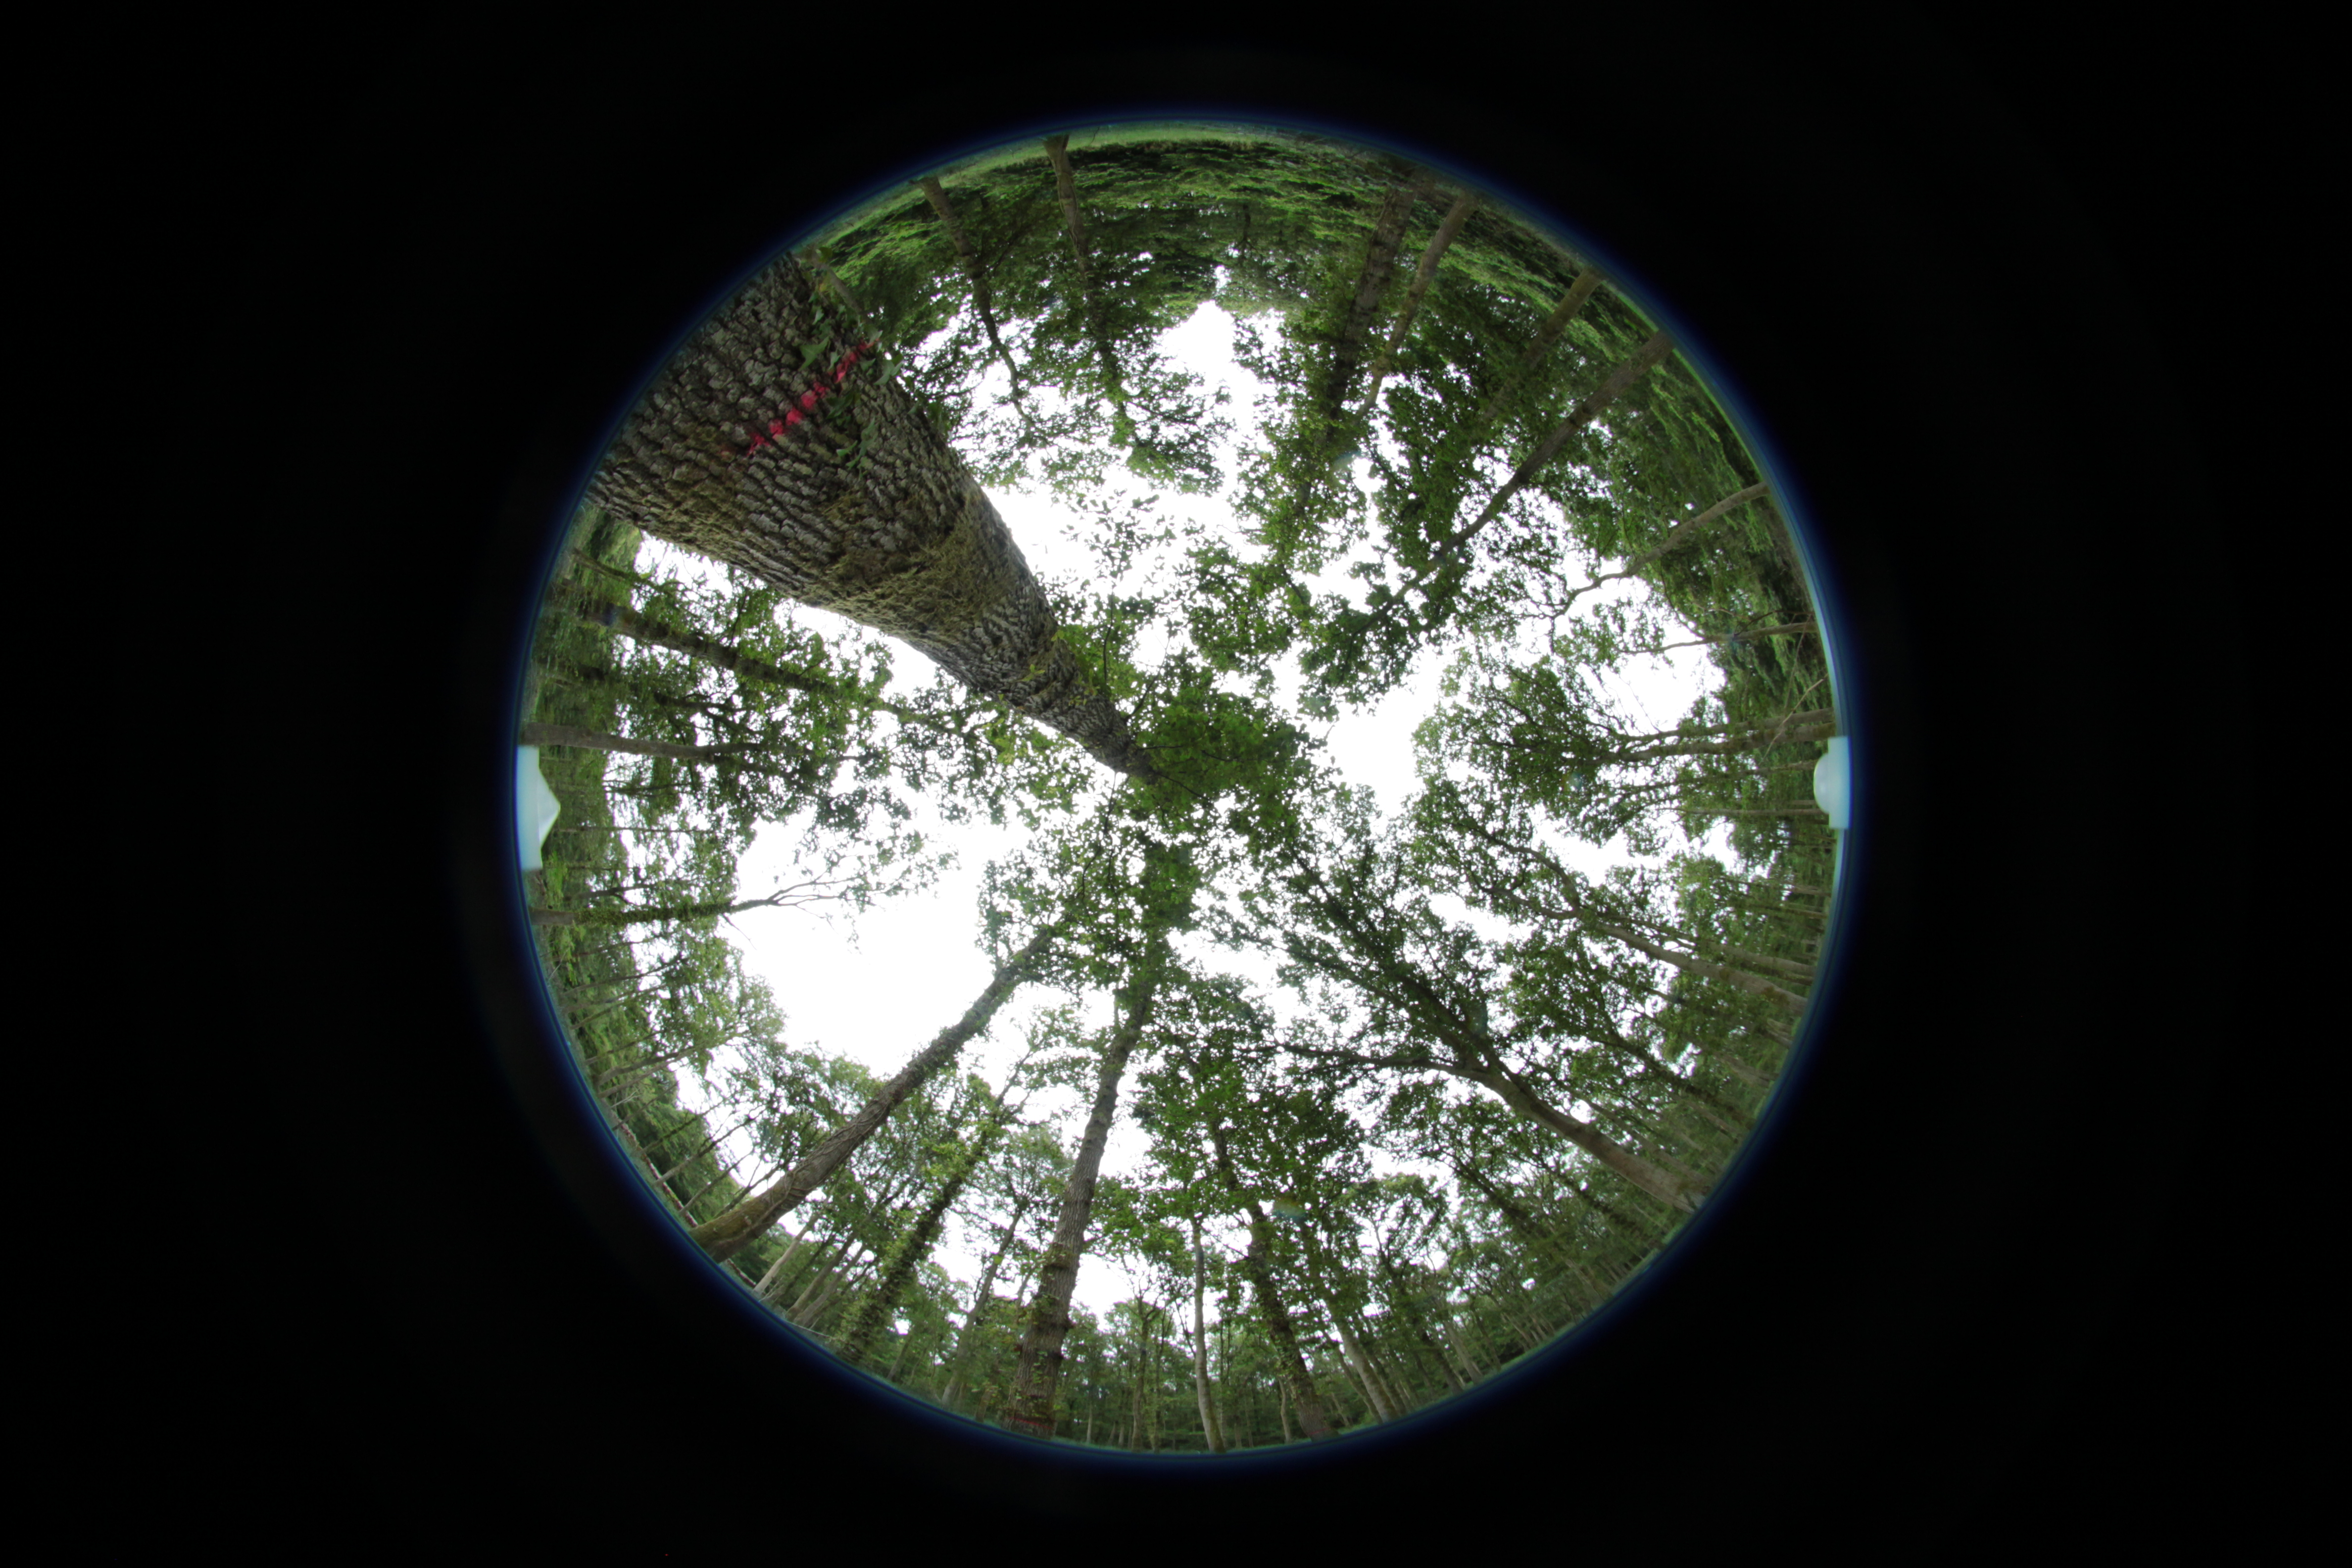
\includegraphics[width=.9\linewidth]{chapter/chapter4/252exp1.jpg}
  \caption{Thinned forest}
  \label{chap4:fig:sub2}
\end{subfigure}
\caption{Hemispherical photographs from the Alice Holt flux site showing the difference between the thinned and unthinned sides of the forest.}
\label{chap4:fig:hemiphotos}
\end{figure}

\subsection{Litter traps}

Finally litter traps were used to find estimates to LAI and leaf mass per area. Here we placed litter traps under the canopy to catch leaf litter as it falls into a bag attached to the bottom of the trap. The bags were changed every week during the litter fall period and the litter sorted into species. Every week the litter was dried in an oven at $70^{\text{o}}\text{C}$ and weighed. This gave us the dry-weight of the leaf litter for the 2015 season. Towards the end of the season we scanned a subsample for each species of 100 leaves to find an area, we then dried and weighed each subsample, a relationship between dry-weight and leaf area was then be built (leaf mass per area) and used to infer the total LAI for each trap once the whole seasons litter has been collected. This method of LAI calculation is the most time consuming.  

A total of six litter traps were established at points along the transects (positions shown in Figure~\ref{chap4:fig:lit_traps}) allowing for comparison with the other methods. The 6 litter traps are not enough to describe the LAI for the research site \citep{kimmins1973some}. We use these litter traps as a point of comparison and validation for the ceptometer and hemispherical photograph estimates of LAI made at the same locations and also for estimates to leaf mass per area. From our litter trap observations we find a leaf mass per area of 29~g~C~m\(^{-2}\) free soluble carbohydrates for both sides of the forest.

\begin{figure}[ht]
    \centering
    \includegraphics[width=0.8\textwidth]{chapter/chapter4/litter_trap.pdf}
    \caption{Litter trap locations for Alice Holt.} \label{chap4:fig:lit_traps}
\end{figure}


\subsection{Comparison of methods} \label{chap4:sec:lai_comp}

In Figure~\ref{chap4:fig:lai_comp07} and \ref{chap4:fig:lai_comp14} we show a comparison of the different methods of estimating LAI for the unthinned and thinned forest respectively. We can see that in all cases LAI derived from the litter traps is always greater than LAI estimated from optical methods, this is expected from previous comparisons \citep{breda2003ground}.
 
Although the ceptometer is the fastest method for measuring LAI it is also the most variable, being extremely sensitive to the solar zenith angle and clear sky conditions. If the sun is low in the sky the radiation will pass through much more photosynthetically active material than if the sun is directly above head, causing spikes in the LAI value. We can see that the LAI estimates from the hemispherical photographs are much less variable than the ceptometer. As discussed in section~\ref{chap4:sec:hemi_photos} the hemispherical estimate is actually of plant area index, as we have not removed trunks and branches from the gap fraction calculation. However, this does not appear to have a great impact on results as hemispherical photograph derived LAI is still the lowest estimate of all three. 

\begin{figure}[ht]
    \centering
    \includegraphics[width=0.8\textwidth]{chapter/chapter4/thinned07.pdf}
    \caption{LAI comparison for unthinned forest. Dots and solid line represent observations made at different points along transects, dotted lines represent the mean of the observations.} \label{chap4:fig:lai_comp07}
\end{figure}

\begin{figure}[ht]
    \centering
    \includegraphics[width=0.8\textwidth]{chapter/chapter4/thinned14.pdf}
    \caption{LAI comparison for thinned forest. Dots and solid line represent observations made at different points along transects, dotted lines represent the mean of the observations.} \label{chap4:fig:lai_comp14}
\end{figure}

\section{Point-centred quater observations}

We used the method of Point-Centred Quarters (PCQ) \citep{dahdouh2006empirical} to determine an estimate of the woody biomass for both unthinned and thinned forest in the Straits Inclosure. The PCQ method is conducted at each sampling point as follows:
\begin{itemize}
\item Using a compass, map 4 regions from the central sampling point
\item Measure the distance from the central sampling point to the nearest tree in each quarter
\item Measure the Diameter at Breast Height (DBH) for each tree (shown in Figure~\ref{chap4:fig:dbh_me}) and record the species 
\end{itemize}
There were 114 points samples along the three transects, from these measurements we derived estimates to tree density and mean DBH for both thinned and unthinned sides of the forest. We then used allometric relationships between DBH and total above ground biomass and coarse root biomass, found in work carried out by Forest Research and in \citet{mckay2003woodfuel}. These relationships were as follows,
\begin{equation}
\text{above ground dry-mass} = 0.0678\times \overline{\text{DBH}}^{2.619}
\end{equation}
and
\begin{equation}
\text{below ground coarse root dry-mass} = 0.149\times \overline{\text{DBH}}^{2.12}.
\end{equation}

This gave us an estimate to the dry-mass in kilograms for the average tree in our sampling area. Assuming that half of all dry-mass is carbon we can find an estimate of total woody and coarse root carbon in g~C~m\(^{-2}\) using the equation,
\begin{multline}
\text{total woody and coarse root carbon} =  \\1000\times0.5\times(\text{above ground dry-mass} + \text{below ground coarse root dry-mass})\times \text{tree density}.
\end{multline}

Forest Research have carried out their own mensuration studies at the site, these have been conducted at the mensuration points shown in Figure~\ref{chap4:fig:transects}. As these plots are included in our transects this means that hopefully our measurements will be comparable with those from Forest Research.  

\begin{figure}[ht]
    \centering
    \includegraphics[width=0.8\textwidth]{chapter/chapter4/dbh_me.pdf}
    \caption{Taking diameter at breast height measurements at Alice Holt.} \label{chap4:fig:dbh_me}
\end{figure}

\section{Flux tower observations and data processing}

Forest Research provided half-hourly raw flux tower data for the Straits Inclosure from January 1999 to December 2015. These consist of the NEE fluxes and meteorological driving data of temperature, irradiance and atmospheric CO\(_{2}\) concentration for use in the DALEC model. The view from the top of the flux tower in the Straits Inclosure can be seen in Figure~\ref{chap4:fig:flux_me}. Forest Research provided this data in the form of multiple excel spreadsheets corresponding to the flux tower measurement record for each year. To prepare this data for use with data assimilation we first had to convert these 16 excel files to one Python readable data file (here we chose NetCDF), this was the further processed. To process the NEE data we first performed \(u^*\) filtering, where any half-hourly flux observation corresponding to a friction velocity of \(0.2~\text{m s}^{-1}\) (this value represents the point at which flux measurements become unreliable and was found by Forest Research) or less were removed from the data set. We then subjected the observations of NEE to quality control procedures similar to those described by \citet{papale2006towards}. For each year of the NEE dataset this procedure involved calculating the standard deviation of both the positive and negative half-hourly observations and then removing any values that were \(\pm 3\) standard deviations away from the yearly positive/negative mean. This was also repeated on a month by month basis. Gap-filling procedures were not applied to the half-hourly NEE dataset so that only true observations were considered for assimilation. To match the time-step of the DALEC model we computed daily NEE observations by taking the mean over the 48 measurements made each day, selecting only days where there was no missing data.  
 

\begin{figure}[ht]
    \centering
    \includegraphics[width=0.8\textwidth]{chapter/chapter4/top_of_flux.pdf}
    \caption{At the top of the Alice Holt flux tower.} \label{chap4:fig:flux_me}
\end{figure}



%\chapter{Conclusions}
%\label{chap:conclusions}
%\thispagestyle{headings}
%\input{chapter/chapter5}

%\appendix
%\chapter{CMIP5 models}
%\label{chap:appendixA}
%\thispagestyle{headings}
%\def\rightmark{\appendixname \ \thechapter: \ Model list}
%\begin{table}[h!]
  %  \footnotesize
  \caption{\label{tab:models_full}The CMIP5 multi-model ensemble official groups, names and ensemble numbers.}
  \centering
  %\vspace{6pt}
  \begin{tabular}{m{6cm}m{5cm}cc} \hline
    \textbf{Modeling Center (or Group)} & \textbf{Model} & \textbf{Experiment} & \textbf{Ensemble} \\ \hline \hline
    \multirow{8}{\linewidth}{Commonwealth Scientific and Industrial Research Organization (CSIRO) and Bureau of Meteorology (BOM), Australia} & \multirow{4}{\linewidth}{ACCESS1.0\\ \citep{Collier2012}} & AMIP & r1i1p1 \\ \cline{3-4}
     &  & Historical & r1i1p1 \\ \cline{3-4}
     &  & RCP4.5 & r1i1p1 \\ \cline{3-4}
     &  & RCP8.5 & r1i1p1 \\ \cline{2-4}
     & \multirow{4}{\linewidth}{ACCESS1.3\\ \citep{Collier2012}} & AMIP & r1i1p1 \\ \cline{3-4}
     &  & Historical & r1i1p1 \\ \cline{3-4}
     &  & RCP4.5 & r1i1p1 \\ \cline{3-4}
     &  & RCP8.5 & r1i1p1 \\ \hline
    \multirow{16}{\linewidth}{Beijing Climate Center, China Meteorological Administration} & \multirow{8}{\linewidth}{BCC-CSM1.1\\ \citep{Xin2013}} & \multirow{3}{*}{AMIP} & r1i1p1 \\
     &  &  & r2i1p1 \\
     &  &  & r3i1p1 \\ \cline{3-4}
     &  & \multirow{3}{*}{Historical} & r1i1p1 \\
     &  &  & r2i1p1 \\
     &  &  & r3i1p1 \\ \cline{3-4}
     &  & RCP4.5 & r1i1p1 \\ \cline{3-4}
     &  & RCP8.5 & r1i1p1 \\ \cline{2-4}
     & \multirow{8}{\linewidth}{BCC-CSM1.1(m)\\ \citep{Xin2013}} & \multirow{3}{*}{AMIP} & r1i1p1 \\
     &  &  & r2i1p1 \\
     &  &  & r3i1p1 \\ \cline{3-4}
     &  & \multirow{3}{*}{Historical} & r1i1p1 \\
     &  &  & r2i1p1 \\
     &  &  & r3i1p1 \\ \cline{3-4}
     &  & RCP4.5 & r1i1p1 \\ \cline{3-4}
     &  & RCP8.5 & r1i1p1 \\ \hline
    \multirow{4}{\linewidth}{College of Global Change and Earth System Science, Beijing Normal University} & \multirow{4}{\linewidth}{BNU-ESM\\ (Atmospheric component: CAM3.5 -- \citealt{Neale2008})} & AMIP & r1i1p1 \\ \cline{3-4}
     &  & Historical & r1i1p1 \\ \cline{3-4}
     &  & RCP4.5 & r1i1p1 \\ \cline{3-4}
     &  & RCP8.5 & r1i1p1 \\ \hline
    \hline \multicolumn{4}{r}{\textit{Continued on next page}} \\ \hline
  \end{tabular}
\end{table}
\begin{table}
  \centering
  \begin{tabular}{m{6cm}m{5cm}cc} \hline
    \multicolumn{4}{c}%
    {\tablename\ \thetable\ -- \textit{Continued from previous page}} \\
    \hline \textbf{Modeling Center (or Group)} & \textbf{Model} & \textbf{Experiment} & \textbf{Ensemble} \\ \hline \hline
    \multirow{7}{\linewidth}{Canadian Centre for Climate Modelling and Analysis} & \multirow{7}{\linewidth}{CanESM2\\ (Atmospheric component: AGCM4 -- based on \citealt{Scinocca2008})} & \multirow{5}{*}{Historical} & r1i1p1 \\
     &  &  & r2i1p1 \\
     &  &  & r3i1p1 \\
     &  &  & r4i1p1 \\
     &  &  & r5i1p1 \\ \cline{3-4}
     &  & RCP4.5 & r1i1p1 \\ \cline{3-4}
     &  & RCP8.5 & r1i1p1 \\ \hline
    \multirow{7}{\linewidth}{National Center for Atmospheric Research} & \multirow{7}{\linewidth}{CCSM4\\ \citep{Gent2011}} & \multirow{4}{*}{AMIP} & r1i1p1 \\
     &  &  & r2i1p1 \\
     &  &  & r3i1p1 \\
     &  &  & r4i1p1 \\ \cline{3-4}
     &  & Historical & r6i1p1 \\ \cline{3-4}
     &  & RCP4.5 & r6i1p1 \\ \cline{3-4}
     &  & RCP8.5 & r6i1p1 \\ \hline
    \multirow{6}{\linewidth}{Centro Euro-Mediterraneo per i Cambiamenti Climatici} & \multirow{6}{\linewidth}{CMCC-CM\\ \citep{Bellucci2012}} & \multirow{3}{*}{AMIP} & r1i1p1 \\
     &  &  & r2i1p1 \\
     &  &  & r3i1p1 \\ \cline{3-4}
     &  & Historical & r1i1p1 \\ \cline{3-4}
     &  & RCP4.5 & r1i1p1 \\ \cline{3-4}
     &  & RCP8.5 & r1i1p1 \\ \hline
    \multirow{13}{\linewidth}{Centre National de Recherches M\'{e}t\'{e}orologiques / Centre Europ\'{e}en de Recherche et Formation Avanc\'{e}es en Calcul Scientifique} & \multirow{13}{\linewidth}{CNRM-CM5\\ \citep{Voldoire2012}} & AMIP & r1i1p1 \\ \cline{3-4}
     &  & \multirow{10}{*}{Historical} & r1i1p1 \\
     &  &  & r2i1p1 \\
     &  &  & r3i1p1 \\
     &  &  & r4i1p1 \\
     &  &  & r5i1p1 \\
     &  &  & r6i1p1 \\
     &  &  & r7i1p1 \\
     &  &  & r8i1p1 \\
     &  &  & r9i1p1 \\
     &  &  & r10i1p1 \\ \cline{3-4}
     &  & RCP4.5 & r1i1p1 \\ \cline{3-4}
     &  & RCP8.5 & r1i1p1 \\ \hline
    \hline \multicolumn{4}{r}{\textit{Continued on next page}} \\ \hline
  \end{tabular}
\end{table}
\begin{table}
  \centering
  \begin{tabular}{m{6cm}m{5cm}cc} \hline
    \multicolumn{4}{c}%
    {\tablename\ \thetable\ -- \textit{Continued from previous page}} \\
    \hline \textbf{Modeling Center (or Group)} & \textbf{Model} & \textbf{Experiment} & \textbf{Ensemble} \\ \hline \hline
    \multirow{40}{\linewidth}{Commonwealth Scientific and Industrial Research Organization in collaboration with Queensland Climate Change Centre of Excellence} & \multirow{40}{\linewidth}{CSIRO-Mk3.6.0\\ \citep{Rotstayn2012}} & \multirow{10}{*}{AMIP} & r1i1p1 \\
     &  &  & r2i1p1 \\
     &  &  & r3i1p1 \\
     &  &  & r4i1p1 \\
     &  &  & r5i1p1 \\
     &  &  & r6i1p1 \\
     &  &  & r7i1p1 \\
     &  &  & r8i1p1 \\
     &  &  & r9i1p1 \\
     &  &  & r10i1p1 \\ \cline{3-4}
     &  & \multirow{10}{*}{Historical} & r1i1p1 \\
     &  &  & r2i1p1 \\
     &  &  & r3i1p1 \\
     &  &  & r4i1p1 \\
     &  &  & r5i1p1 \\
     &  &  & r6i1p1 \\
     &  &  & r7i1p1 \\
     &  &  & r8i1p1 \\
     &  &  & r9i1p1 \\
     &  &  & r10i1p1 \\ \cline{3-4}
     &  & \multirow{10}{*}{RCP4.5} & r1i1p1 \\
     &  &  & r2i1p1 \\
     &  &  & r3i1p1 \\
     &  &  & r4i1p1 \\
     &  &  & r5i1p1 \\
     &  &  & r6i1p1 \\
     &  &  & r7i1p1 \\
     &  &  & r8i1p1 \\
     &  &  & r9i1p1 \\
     &  &  & r10i1p1 \\ \cline{3-4}
     &  & \multirow{10}{*}{RCP8.5} & r1i1p1 \\
     &  &  & r2i1p1 \\
     &  &  & r3i1p1 \\
     &  &  & r4i1p1 \\
     &  &  & r5i1p1 \\
     &  &  & r6i1p1 \\
     &  &  & r7i1p1 \\
     &  &  & r8i1p1 \\
     &  &  & r9i1p1 \\
     &  &  & r10i1p1 \\ \hline
    \multirow{7}{\linewidth}{EC-EARTH Consortium} & \multirow{7}{\linewidth}{EC-EARTH\\\citep{Sterl2011}} & AMIP & r1i1p1 \\ \cline{3-4}
     &  & Historical & r9i1p1 \\ \cline{3-4}
     &  & \multirow{2}{*}{RCP4.5} & r8i1p1 \\
     &  &  & r12i1p1 \\ \cline{3-4}
     &  & \multirow{3}{*}{RCP8.5} & r6i1p1 \\
     &  &  & r8i1p1 \\
     &  &  & r12i1p1 \\ \hline
    \hline \multicolumn{4}{r}{\textit{Continued on next page}} \\ \hline
  \end{tabular}
\end{table}
\begin{table}
  \centering
  \begin{tabular}{m{6cm}m{5cm}cc} \hline
    \multicolumn{4}{c}%
    {\tablename\ \thetable\ -- \textit{Continued from previous page}} \\
    \hline \textbf{Modeling Center (or Group)} & \textbf{Model} & \textbf{Experiment} & \textbf{Ensemble} \\ \hline \hline
    \multirow{4}{\linewidth}{LASG, Institute of Atmospheric Physics, Chinese Academy of Sciences and CESS, Tsinghua University} & \multirow{4}{\linewidth}{FGOALS-g2\\ \citep{Wang2013}} & AMIP & r1i1p1 \\ \cline{3-4}
     &  & Historical & r3i1p1 \\ \cline{3-4}
     &  & RCP4.5 & r1i1p1 \\ \cline{3-4}
     &  & RCP8.5 & r1i1p1 \\ \hline
    \multirow{13}{\linewidth}{LASG, Institute of Atmospheric Physics, Chinese Academy of Sciences} & \multirow{12}{\linewidth}{FGOALS-s2\\ \citep{Bao2013}} & \multirow{3}{*}{AMIP} & r1i1p1 \\
     &  &  & r2i1p1 \\
     &  &  & r3i1p1 \\ \cline{3-4}
     &  & \multirow{3}{*}{Historical} & r1i1p1 \\
     &  &  & r2i1p1 \\
     &  &  & r3i1p1 \\ \cline{3-4}
     &  & \multirow{3}{*}{RCP4.5} & r1i1p1 \\
     &  &  & r2i1p1 \\
     &  &  & r3i1p1 \\ \cline{3-4}
     &  & \multirow{3}{*}{RCP8.5} & r1i1p1 \\
     &  &  & r2i1p1 \\
     &  &  & r3i1p1 \\ \hline
    \multirow{15}{\linewidth}{NOAA Geophysical Fluid Dynamics Laboratory} & \multirow{9}{\linewidth}{GFDL-CM3\\ (Atmospheric component -- \citealt{Donner2011})} & \multirow{5}{*}{Historical} & r1i1p1 \\
     &  &  & r2i1p1 \\
     &  &  & r3i1p1 \\
     &  &  & r4i1p1 \\
     &  &  & r5i1p1 \\ \cline{3-4}
     &  & \multirow{3}{*}{RCP4.5} & r1i1p1 \\
     &  &  & r3i1p1 \\
     &  &  & r5i1p1 \\ \cline{3-4}
     &  & RCP8.5 & r1i1p1 \\ \cline{2-4}
     & \multirow{3}{\linewidth}{GFDL-ESM2G\\ \citep{Dunne2012,Dunne2013}} & Historical & r1i1p1 \\ \cline{3-4}
     &  & RCP4.5 & r1i1p1 \\ \cline{3-4}
     &  & RCP8.5 & r1i1p1 \\ \cline{2-4}
     & \multirow{3}{\linewidth}{GFDL-ESM2M\\ \citep{Dunne2012,Dunne2013}} & Historical & r1i1p1 \\ \cline{3-4}
     &  & RCP4.5 & r1i1p1 \\ \cline{3-4}
     &  & RCP8.5 & r1i1p1 \\ \hline
    \multirow{15}{\linewidth}{Met Office Hadley Centre} & \multirow{7}{\linewidth}{HadGEM2-A\\ \citep{Bellouin2011}} & \multirow{7}{*}{AMIP} & r1i2p1 \\
     &  &  & r2i3p1 \\
     &  &  & r3i2p1 \\
     &  &  & r4i3p1 \\
     &  &  & r5i2p1 \\
     &  &  & r6i3p1 \\
     &  &  & r7i2p1 \\ \cline{2-4}
     & \multirow{5}{\linewidth}{HadGEM2-CC\\ \citep{Bellouin2011}} & \multirow{2}{*}{Historical} & r1i1p1 \\
     &  &  & r2i1p1 \\ \cline{3-4}
     &  & RCP4.5 & r1i1p1 \\ \cline{3-4}
     &  & \multirow{2}{*}{RCP8.5} & r1i1p1 \\
     &  &  & r2i1p1 \\ \cline{2-4}
     & \multirow{3}{\linewidth}{HadGEM2-ES\\ \citep{Bellouin2011}} & Historical & r1i1p1 \\ \cline{3-4}
     &  & RCP4.5 & r1i1p1 \\ \cline{3-4}
     &  & RCP8.5 & r1i1p1 \\ \hline
    \hline \multicolumn{4}{r}{\textit{Continued on next page}} \\ \hline
  \end{tabular}
\end{table}
\begin{table}
  \centering
  \begin{tabular}{m{6cm}m{5cm}cc} \hline
    \multicolumn{4}{c}%
    {\tablename\ \thetable\ -- \textit{Continued from previous page}} \\
    \hline \textbf{Modeling Center (or Group)} & \textbf{Model} & \textbf{Experiment} & \textbf{Ensemble} \\ \hline \hline
    \multirow{4}{\linewidth}{Institute for Numerical Mathematics} & \multirow{4}{\linewidth}{INM-CM4\\ \citep{Volodin2010}} & AMIP & r1i1p1 \\ \cline{3-4}
     &  & Historical & r1i1p1 \\ \cline{3-4}
     &  & RCP4.5 & r1i1p1 \\ \cline{3-4}
     &  & RCP8.5 & r1i1p1 \\ \hline
    \multirow{29}{\linewidth}{Institut Pierre-Simon Laplace} & \multirow{18}{\linewidth}{IPSL-CM5A-LR\\ (\citealt{Dufresne2013}; Atmospheric component: LMDZ5A -- \citealt{Hourdin2012})} & \multirow{6}{*}{AMIP} & r1i1p1 \\
     &  &  & r2i1p1 \\
     &  &  & r3i1p1 \\
     &  &  & r4i1p1 \\
     &  &  & r5i1p1 \\
     &  &  & r6i1p1 \\ \cline{3-4}
     &  & \multirow{4}{*}{Historical} & r1i1p1 \\
     &  &  & r2i1p1 \\
     &  &  & r3i1p1 \\
     &  &  & r4i1p1 \\ \cline{3-4}
     &  & \multirow{4}{*}{RCP4.5} & r1i1p1 \\
     &  &  & r2i1p1 \\
     &  &  & r3i1p1 \\
     &  &  & r4i1p1 \\ \cline{3-4}
     &  & \multirow{4}{*}{RCP8.5} & r1i1p1 \\
     &  &  & r2i1p1 \\
     &  &  & r3i1p1 \\
     &  &  & r4i1p1 \\ \cline{2-4}
     & \multirow{4}{\linewidth}{IPSL-CM5A-MR\\ (\citealt{Dufresne2013}; Atmosphere: LMDZ5A -- \citealt{Hourdin2012})} & AMIP & r1i1p1 \\ \cline{3-4}
     &  & Historical & r1i1p1 \\ \cline{3-4}
     &  & RCP4.5 & r1i1p1 \\ \cline{3-4}
     &  & RCP8.5 & r1i1p1 \\ \cline{2-4}
     & \multirow{7}{\linewidth}{IPSL-CM5B-LR\\ (\citealt{Dufresne2013}; Atmospheric component: LMDZ5A -- \citealt{Hourdin2012a,Rio2012})} & \multirow{3}{*}{AMIP} & r1i1p1 \\
     &  &  & r2i1p1 \\
     &  &  & r3i1p1 \\ \cline{3-4}
     &  & \multirow{2}{*}{Historical} & r1i1p1 \\
     &  &  & r2i1p1 \\ \cline{3-4}
     &  & RCP4.5 & r1i1p1 \\ \cline{3-4}
     &  & RCP8.5 & r1i1p1 \\ \hline
    \multirow{8}{\linewidth}{Japan Agency for Marine-Earth Science and Technology, Atmosphere and Ocean Research Institute (The University of Tokyo), and National Institute for Environmental Studies} & \multirow{5}{\linewidth}{MIROC-ESM\\ \citep{Watanabe2011}} & \multirow{3}{*}{Historical} & r1i1p1 \\
     &  &  & r2i1p1 \\
     &  &  & r3i1p1 \\ \cline{3-4}
     &  & RCP4.5 & r1i1p1 \\ \cline{3-4}
     &  & RCP8.5 & r1i1p1 \\ \cline{2-4}
     & \multirow{3}{\linewidth}{MIROC-ESM-CHEM\\ \citep{Watanabe2011}} & Historical & r1i1p1 \\ \cline{3-4}
     &  & RCP4.5 & r1i1p1 \\ \cline{3-4}
     &  & RCP8.5 & r1i1p1 \\ \hline
    \hline \multicolumn{4}{r}{\textit{Continued on next page}} \\ \hline
  \end{tabular}
\end{table}
\begin{table}
  \centering
  \begin{tabular}{m{6cm}m{5cm}cc} \hline
    \multicolumn{4}{c}%
    {\tablename\ \thetable\ -- \textit{Continued from previous page}} \\
    \hline \textbf{Modeling Center (or Group)} & \textbf{Model} & \textbf{Experiment} & \textbf{Ensemble} \\ \hline \hline
    \multirow{12}{\linewidth}{Atmosphere and Ocean Research Institute (The University of Tokyo), and National Institute for Environmental Studies, and Japan Agency for Marine-Earth Science and Technology} & \multirow{12}{\linewidth}{MIROC5\\ \citep{Watanabe2010}} & \multirow{2}{*}{AMIP} & r1i1p1 \\
     &  &  & r2i1p1 \\ \cline{3-4}
     &  & \multirow{4}{*}{Historical} & r1i1p1 \\
     &  &  & r2i1p1 \\
     &  &  & r3i1p1 \\
     &  &  & r4i1p1 \\ \cline{3-4}
     &  & \multirow{3}{*}{RCP4.5} & r1i1p1 \\
     &  &  & r2i1p1 \\
     &  &  & r3i1p1 \\ \cline{3-4}
     &  & \multirow{3}{*}{RCP8.5} & r1i1p1 \\
     &  &  & r2i1p1 \\
     &  &  & r3i1p1 \\ \hline
    \multirow{20}{\linewidth}{Max-Planck-Institut f\"{u}r Meteorologie (Max Planck Institute for Meteorology)} & \multirow{12}{\linewidth}{MPI-ESM-LR\\ (\citealt{Mauritsen2012}; Atmospheric component: ECHAM6 -- \citealt{Stevens2013})} & \multirow{3}{*}{AMIP} & r1i1p1 \\
     &  &  & r2i1p1 \\
     &  &  & r3i1p1 \\ \cline{3-4}
     &  & \multirow{3}{*}{Historical} & r1i1p1 \\
     &  &  & r2i1p1 \\
     &  &  & r3i1p1 \\ \cline{3-4}
     &  & \multirow{3}{*}{RCP4.5} & r1i1p1 \\
     &  &  & r2i1p1 \\
     &  &  & r3i1p1 \\ \cline{3-4}
     &  & \multirow{3}{*}{RCP8.5} & r1i1p1 \\
     &  &  & r2i1p1 \\
     &  &  & r3i1p1 \\ \cline{2-4}
     & \multirow{8}{\linewidth}{MPI-ESM-MR\\ (\citealt{Mauritsen2012}; Atmospheric component: ECHAM6 -- \citealt{Stevens2013})} & \multirow{3}{*}{AMIP} & r1i1p1 \\
     &  &  & r2i1p1 \\
     &  &  & r3i1p1 \\ \cline{3-4}
     &  & \multirow{3}{*}{Historical} & r1i1p1 \\
     &  &  & r2i1p1 \\
     &  &  & r3i1p1 \\ \cline{3-4}
     &  & RCP4.5 & r1i1p1 \\ \cline{3-4}
     &  & RCP8.5 & r1i1p1 \\ \hline
    \multirow{10}{\linewidth}{Meteorological Research Institute} & \multirow{10}{\linewidth}{MRI-CGCM3\\ \citep{Yukimoto2012}} & \multirow{3}{*}{AMIP} & r1i1p1 \\
     &  &  & r2i1p1 \\
     &  &  & r3i1p1 \\ \cline{3-4}
     &  & \multirow{5}{*}{Historical} & r1i1p1 \\
     &  &  & r2i1p1 \\
     &  &  & r3i1p1 \\
     &  &  & r4i1p2 \\
     &  &  & r5i1p2 \\ \cline{3-4}
     &  & RCP4.5 & r1i1p1 \\ \cline{3-4}
     &  & RCP8.5 & r1i1p1 \\ \hline
    \multirow{8}{\linewidth}{Norwegian Climate Centre} & \multirow{8}{\linewidth}{NorESM1-M\\ \citep{Bentsen2012,Iversen2013}} &  \multirow{3}{*}{AMIP} & r1i1p1 \\
     &  &  & r2i1p1 \\
     &  &  & r3i1p1 \\ \cline{3-4}
     &  & \multirow{3}{*}{Historical} & r1i1p1 \\
     &  &  & r2i1p1 \\
     &  &  & r3i1p1 \\ \cline{3-4}
     &  & RCP4.5 & r1i1p1 \\ \cline{3-4}
     &  & RCP8.5 & r1i1p1 \\ \hline \hline
  \end{tabular}
\end{table}


\newpage
\addcontentsline{toc}{chapter}{Bibliography}
\def\rightmark{Bibliography}
\def\leftmark{Bibliography}
\renewcommand*{\bibname}{\centerline{\Huge{\bfseries{\scshape{Bibliography}}}}}
\bibliography{./library}
\bibliographystyle{./ametsoc}

\end{document}
